
\chapter{Special Elements} \label{SpecElem}

One advantage of SixTrack, that has been adopted from RACETRACK\index{RACETRACK}, is that it easily allows to define elements for a specific purpose.\index{special elements}
The special elements implemented util now are found in this section.
All Special Elements should be written in the \texttt{fort.3} file.\index{fort.3}

% ================================================================================================================================ %
\section{Multipole Coefficients} \label{MulCoe}

Sets of normal and skew multipoles of up to tenth order, each with an r.m.s. value, can be combined with this block.\index{multipole coefficients}\index{MULT}
The multipole kick is calculated using a Horner scheme\index{Horner scheme}, which saves considerably in computation time.
Moreover, using the multipole block reduces the number of elements in the single element list (\ref{SinEle})\index{single elements}.

\bigskip
\begin{tabular}{@{}lp{0.8\linewidth}}
    \textbf{Keyword}    & \texttt{MULT}\index{MULT} \\
    \textbf{Data lines} & 2 to 12 \\
    \textbf{Format}     & First line: \texttt{name $R_{0}$ $\delta_{0}$}. \\
                        & Lines 2 to 12: \texttt{$B_{n}$ rms-$B_{n}$ $A_{n}$ rms-$A_{n}$}.
\end{tabular}

\paragraph{Format Description}~

\bigskip
\begin{tabular}{@{}lp{0.8\linewidth}}
    \texttt{name}    & Name of the multipole block which must appear in the list of single elements\index{single elements} (\ref{MulBlo}). \\
    \texttt{$R_{0}$} & Reference radius (in mm) at which the magnet errors are calculated. This makes it convenient to use values from field measurements. \\
    \texttt{$\delta_{0}$} & Bending strength\index{bending strength} of the dipole (in mrad). Field errors\index{field errors} of line 2--11 are taken to be relative to the bending strength.
\end{tabular}

\paragraph{Remarks}
\begin{enumerate}
    \item The $B_{n}$ and $A_{n}$ are related to the $b_{n}, a_{n}$ of the single nonlinear element (\ref{NonEle}) in the following way:
        \begin{align*}
            b_{n} &= \delta_{0} B_{n} R_{0}^{1-n} 10^{3n-6} \\
            a_{n} &= \delta_{0} A_{n} R_{0}^{1-n} 10^{3n-6}
        \end{align*}
    \item The sign convention and the factorial ($n$!) are treated as for the single non-linear elements in (\ref{NonEle}).
    \item Multipoles of different names can be set to be equal using the \texttt{ORG} input block.
    \item 22-poles are included ($n=11$). By enlarging the parameter \texttt{MMUL} (Appendix~\ref{DSP}) up to 40-poles (\texttt{MMUL=20})\index{MMUL} can be treated. To make the change of \texttt{MMUL} effective, it is of course necessary to recompile the program.
\end{enumerate}

\section{Generalized RF-Multipoles} \label{generalrf}

\bigskip
\begin{tabular}{@{}lp{0.8\linewidth}}
    \textbf{Keyword}    & \texttt{RFMU}\index{RFMU} \\
    \textbf{Data lines} & 2 to 21 \\
    \textbf{Format}     & First line: \texttt{name frequency}  . \\
                        & Lines 2 to 21: \texttt{$B_{n}$ $\phi_{Bn}$ $A_{n}$ $\phi_{An}$}.
\end{tabular}

\paragraph{Format Description}~

\bigskip
\begin{tabular}{@{}lp{0.8\linewidth}}
    \texttt{name}    & Name of the block which must appear in the list of single elements\index{single elements} (\ref{rfmulbloc}). \\
    \texttt{$B_{n}$} & Strength of the normal multipole of order n.  \\
    \texttt{$\phi_{Bn}$} & Phase (in radians) of the normal multipole of order n.  \\
    \texttt{$A_{n}$} & Strength of the skew multipole of order n.  \\
    \texttt{$\phi_{An}$} & Phase (in radians) of the skew multipole of order n.  \\
\end{tabular}

% ================================================================================================================================ %
\section{Aperture Limitations} \label{ApeLim}
The aperture LIMItation block allows to define aperture limitations in the machine and hence describe the mechanical acceptance of the machine.\index{aperture limit}\index{LIMI}
In this way, it is possible to check if particles being tracked still remain inside the machine mechanical aperture or will be lost against the beam pipe.

In addition to the check against the detailed model of the machine, there is also a general (rectangular) aperture check at each non-zero length element.
The general aperture check is always on, but in general values of the specifiers are set large enough (\ref{T-DTP}) to define the short term dynamic aperture and be outside of any factual machine mechanical aperture.

\subsection{General Description} \label{ApeLim:GenDesc}
Each non-linear (zero length) element defined in the \textit{Single Element} input block (\ref{NonEle}) except multipole blocks (\ref{MulBlo}) can be used to define aperture limitations, but it is highly recommended to use dedicated markers.
Several aperture types are available to the user (see later).

The aperture limitations are taken into account during tracking by the online aperture checking algorithm, which verifies that the tracked particles falls within the mechanical acceptance of the machine.
When a particle does not fit into the mechanical acceptance, it is removed from tracking; its coordinates at the point of loss are reported in a text file.
A back-tracking algorithm finds the actual loss location interpolating the aperture profile by means of a bi-section method; the user can set the precision with which the longitudinal position is found (default is 10~cm).
While on by default, the algorithm can be switched off by the user; in this case, the particle coordinates reported in the loss file are those at the aperture marker where the particle is found out of the mechanical aperture of the machine.
Particles outside of the mechanical acceptance will be mercilessly killed, unless explicitly requested by the user (see Sec.~\ref{ApeLim:inpOptions}).

The present implementation extends the functionalities developed in the context of the Fluka-SixTrack coupling~\cite{coupling:1,coupling:2}.
Please note that, if aperture markers are defined in the \texttt{LIMI} block, the aperture check is triggered only by the markers.
On the other hand, the general aperture check is performed at every element and it is always on.
Finally, no matter if the \texttt{LIMI} block is present or not, or if the back-tracking algorithm is on or off, SixTrack dumps all particles at their loss point in the \texttt{aperture\_losses.dat} file (see Sec.~\ref{ApeLim:ApeLossesFileFormat}).

\newpage
\paragraph{Format Description}~

\bigskip
\begin{tabular}{@{}lp{0.8\linewidth}}
    \textbf{Keyword}    & \texttt{LIMI}\index{LIMI} \\
    \textbf{Data lines} & Variable \\
    \textbf{Format}     & Each aperture marker is fully specified by means of its type and
                          numerical parameters (see Sec.~\ref{ApeLim:ApeSpecs}).
                          Other input options are available to the user,
                          headed by specific keywords, to control the respective parameters.
\end{tabular}

\bigskip
\subsection{Specifying Aperture Marker}\label{ApeLim:ApeSpecs}
An aperture profile can be assigned to a SINGLE ELEMENT specifying its type and numerical specifiers:

\paragraph{Format:}
\texttt{name type aper\_1 aper\_2 aper\_3 aper\_4 x\_off y\_off angle}

\begin{longtabu}{@{}lp{0.8\linewidth}}
    \texttt{name}   & The name of any non-linear (zero length) element in the \textit{Single Element} input block~(\ref{NonEle}) except multipole blocks~(\ref{MulBlo}). \\
    \texttt{type}   & Type of aperture limitation (string). See Tab.~\ref{tab:apeSpecs} for the types
                      presently available. \\
    \texttt{aper\_1} to \texttt{aper\_4}  & Aperture specifiers (floats).
                      Their actual meaning depend on the aperture type. The aperture specifiers are
                      aligned to those of MAD-X~\cite{MAD}, with the exception of the Racetrack,
                      that can have an ellyptical corner. See Tab.~\ref{tab:apeSpecs} for their
                      meanings. Only the Transition type needs 8 specifiers (hence from \texttt{aper\_1} to \texttt{aper\_8}). \\
    \texttt{x\_off} and \texttt{y\_off}  & Hor.~and ver.~offsets in mm. \\
    \texttt{angle}  & Tilt angle is in degrees. The tilt is around the offset point.\\
\end{longtabu}

The last three numerical specifiers are optional, whereas the others are mandatory, depending on the type.
Tab.~\ref{tab:apeSpecs} summarises the aperture types presently available and the meaning of the respective numerical specifiers; see also Fig.~\ref{fig:APE_sketch} for further geometrical clarifications.
The list of aperture markers and specifiers can be given directly in the \texttt{fort.3} file, in the \texttt{LIMI} block, or via a text file, the name of which must be specified in the \texttt{LIMI} block with the \texttt{LOAD} keyword (see Sec.~\ref{ApeLim:inpOptions}).
For the convention on signs for the last three (optional) aperture specifiers, please see Fig.~\ref{fig:oct_sketch}.

\begin{center}
\begin{longtable}{|c|c|c|c|}%{|p{2.0cm} | p{1.2cm} | p{1.0cm} | p{9.0cm}|}
    %Note: \\* (with the star) used to inhibit page breaks in the middle of groups of the same type
    \caption{Aperture types and specifiers. Only the mandatory specifiers are reported.}
    \label{tab:apeSpecs} \\*
    \hline
    \rowcolor{blue!30}
    & & \multicolumn{2}{|c|}{Aperture specifier} \\*
    \rowcolor{blue!30}
    Name & \texttt{Type} & name & meaning \\*
    \hline
    \endfirsthead

    Circle  & \texttt{CR} & \texttt{aper\_1} & radius [mm] \\*
    \hline

    Rectangle & \texttt{RE} & \texttt{aper\_1} & hor.~half-size [mm] \\*
    & & \texttt{aper\_2} & ver.~half-size [mm] \\*
    \hline

    Ellipse & \texttt{EL} & \texttt{aper\_1} & hor.~semi-axis [mm] \\*
    & & \texttt{aper\_2} & ver.~semi-axis [mm] \\*
    \hline

    RectEllipse & \texttt{RL} & \texttt{aper\_1} & hor.~half-size [mm] \\*
    & & \texttt{aper\_2} & ver.~half-size [mm] \\*
    & & \texttt{aper\_3} & hor.~semi-axis [mm] \\*
    & & \texttt{aper\_4} & ver.~semi-axis [mm] \\*
    \hline

    Octagon & \texttt{OC} & \texttt{aper\_1} & hor.~position of ver.~side [mm] \\*
    & & \texttt{aper\_2} & ver.~position of hor.~side [mm] \\*
    & & \texttt{aper\_3} & angle of first cut corner [degree] \\*
    & & \texttt{aper\_4} & angle of second cut corner [degree] \\*
    \hline

    Ractetrack & \texttt{RT} & \texttt{aper\_1} & hor.~displ.~of ellypse centre [mm] \\*
    & & \texttt{aper\_2} & ver.~displ.~of ellypse centre [mm] \\*
    & & \texttt{aper\_3} & hor.~semi-axis [mm] \\*
    & & \texttt{aper\_4} & ver.~semi-axis [mm] \\*
    \hline

    Transition & \texttt{TR} & \texttt{aper\_1} & hor.~half-size [mm] \\*
    & & \texttt{aper\_2} & ver.~half-size [mm] \\*
    & & \texttt{aper\_3} & hor.~semi-axis [mm] \\*
    & & \texttt{aper\_4} & ver.~semi-axis [mm] \\*
    & & \texttt{aper\_5} & hor.~displ.~of ellypse centre (a-la RACETRACK) [mm] \\*
    & & \texttt{aper\_6} & hor.~displ.~of ellypse centre (a-la RACETRACK) [mm] \\*
    & & \texttt{aper\_7} & angle of first cut corner [rad] \\*
    & & \texttt{aper\_8} & angle of second cut corner [rad] \\*
    \hline

%     \rowcolor{blue!15}
%     \multicolumn{4}{|l|}{Type specific parameters} \\*
%     \texttt{GAUSSIAN} & \texttt{$\sigma$} & mm & Sigma of the e--beam.\\*
\end{longtable}
\end{center}

\begin{figure}
\centering
\begin{minipage}{.555\textwidth}
  \centering
  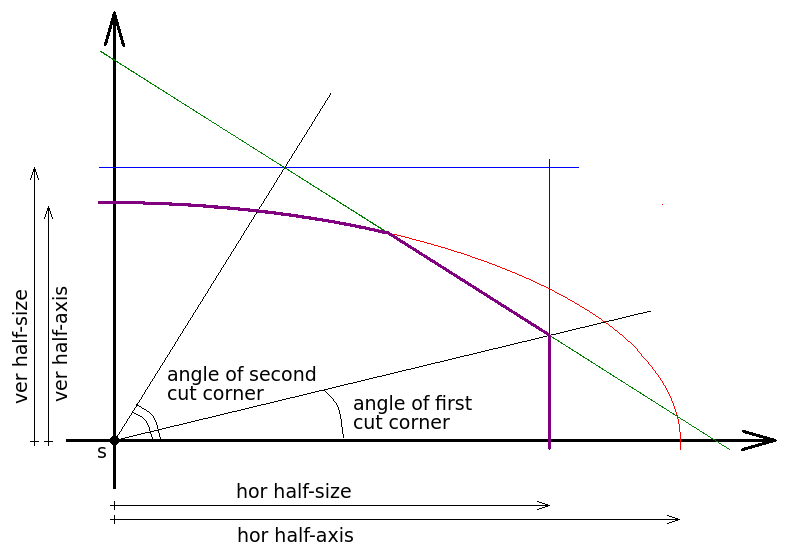
\includegraphics[width=0.95\linewidth]{figures/apertureSketch.png}
  \captionof{figure}{Sketch of the most general aperture profile currently treated by the aperture module. The purple line marks the actual aperture restriction as interpreted by the code with the given parameters.}
  \label{fig:APE_sketch}
\end{minipage}
\hfill
\begin{minipage}{.425\textwidth}
  \centering
  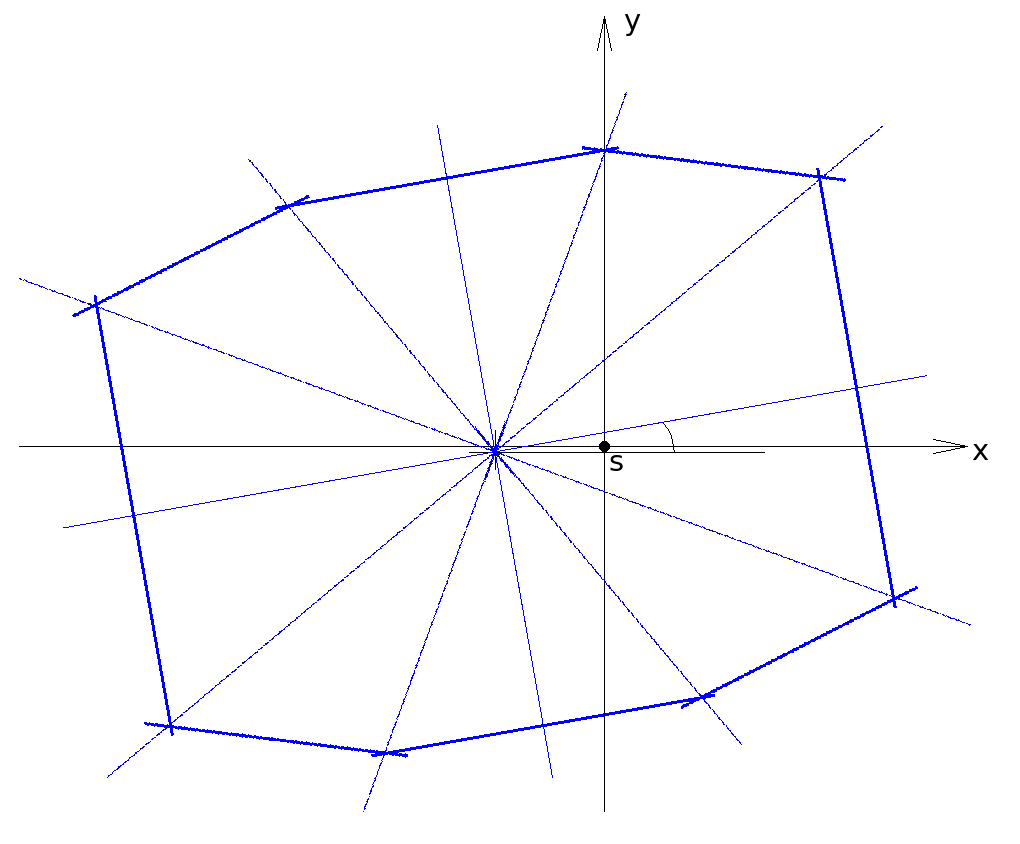
\includegraphics[width=0.95\linewidth]{figures/OctExSketch.png}
  \captionof{figure}{Sketch of the octagon aperture shown in the example. While both offsets are negative,
  the tilt angle is positive.}
  \label{fig:oct_sketch}
\end{minipage}
\end{figure}

\bigskip
\subsection{Other Input Options}\label{ApeLim:inpOptions}
The user can customize the behavior of the \texttt{LIMI} block concerning the back-tracking algorithm. The syntax is via keywords, followed by positional arguments.
Tab.~\ref{tab:apeInpOptions} lists all available options, their syntax and meaning.

\begin{center}
\begin{longtable}{|c|c|l|}%{|p{2.0cm} | p{1.2cm} | p{1.0cm} | p{9.0cm}|}
    %Note: \\* (with the star) used to inhibit page breaks in the middle of groups of the same type
    \caption{Other input options of the \texttt{LIMI} block. Options are listed in alphabetical order.}
    \label{tab:apeInpOptions} \\*
    \hline
    \rowcolor{blue!30}
    keyword & argument & description \\*
    \hline
    \endfirsthead

    \texttt{BACKTRKOFF} & \multicolumn{2}{l|}{to disable back-tracking.} \\*
                        & \multicolumn{2}{l|}{Consequently, particle losses will occur only at aperture markers.} \\*
    \hline

    \texttt{DEBUG} & \multicolumn{2}{l|}{to enable debugging output for the aperture code.} \\*
                   & \multicolumn{2}{l|}{For the moment, this flag only increase the verbosity during parsing of \texttt{fort.3}.} \\*
    \hline

    \texttt{LOAD}  & \multicolumn{2}{l|}{to load specifications of apertures from a file.} \\*
    \cline{2-3}
                   & filename & ASCII file containing the specifications of apertures \\*
    \hline

    \texttt{PREC}  & \multicolumn{2}{l|}{to set custom accuracy in finding the actual loss location} \\*
    \cline{2-3}
                   & precision & precision of back-tracking [m] \\*
    \hline

    \texttt{PRIN}  & \multicolumn{2}{l|}{to echo the profile of the machine aperture with $s$ to a file.} \\*
                   & \multicolumn{2}{l|}{The precision set for back-tracking is used also as precision of the echo.} \\*
    \cline{2-3}
                   & filename & ASCII file where to echo the machine aperture \\*
                   & \texttt{MEM} & optional flag to dump aperture profile as in memory \\*
    \hline

    \texttt{SAVE}  & \multicolumn{2}{l|}{to avoid killing particles out of the mechanical aperture.} \\*
                   & \multicolumn{2}{l|}{Use this option for direct comparisons against \texttt{BeamLossPattern} profiles.} \\*
    \hline

    \texttt{XSEC}  & \multicolumn{2}{l|}{to dump aperture cross sections at specific $s$-locations} \\*
                   & \multicolumn{2}{l|}{(NOT OPERATIONAL YET!)} \\*
    \cline{2-3}
                   & filename & ASCII file where to echo the cross section \\*
                   & $s_{\textrm{min}}$ & first $s$-location where to get the cross-section [m] \\*
                   & $s_{\textrm{max}}$ & last $s$-location where to get the cross-section [m] (optional) \\*
                   & $\Delta s$ & longitudinal steps where to calculate the cross-section [m] (optional) \\*
                   & N & number of azimuthal angles (optional) \\*
    \hline

%     \rowcolor{blue!15}
%     \multicolumn{4}{|l|}{Type specific parameters} \\*
%     \texttt{GAUSSIAN} & \texttt{$\sigma$} & mm & Sigma of the e--beam.\\*
\end{longtable}
\end{center}

\subsection{Format of \texttt{aperture\_losses.dat} File}\label{ApeLim:ApeLossesFileFormat}
The \texttt{aperture\_losses.dat} file lists all lost particles, along with their coordinates at the loss point.
The file is generated no matter if the \texttt{LIMI} block has been inserted in the \texttt{fort.3} or not, or if the back-tracking algorithm is on or off.
Table~\ref{tab:apeLossesFileFormat} shows the format of the file.
If the code is compiled with the \texttt{FLUKA} compilation flag, the particle ID is complemented by the parent particle ID and the statistical weight.

\begin{center}
\begin{longtable}{|l|l|}%{|p{2.0cm} | p{1.2cm} | p{1.0cm} | p{9.0cm}|}
    %Note: \\* (with the star) used to inhibit page breaks in the middle of groups of the same type
  \caption{Columns of the \texttt{aperture\_losses.dat} file. The number between
    parentheses refers to the case SixTrack is compiled for coupling to Fluka, i.e.~if
    the \texttt{FLUKA} compilation flag is on. A '-' means that a given column is
    not available when SixTrack is compiled the \texttt{FLUKA} compilation flag.}
    \label{tab:apeLossesFileFormat} \\*
    \hline
    \rowcolor{blue!30}
    \# & Description \\*
    \hline
    \endfirsthead

    1  & turn number \\*
    2  & index of entry in accelerator sequence \\*
    3  & index of element in the SINGLE ELEMENT array \\*
    4  & name of SINGLE ELEMENT \\*
    5  & $s$-coordinate of loss point [m] \\*
    6  & particle id \\*
    -   (7) & parent particle id \\*
    -   (8) & statistical weight \\*
    7   (9) & $x$ at loss point [m] \\*
    8  (10) & $x'$ at loss point [] \\*
    9  (11) & $y$ at loss point [m] \\*
    10 (12) & $y'$ at loss point [] \\*
    11 (13) & linear momentum [GeV/c] \\*
    12 (14) & energy deviation [eV] \\*
    13 (15) & time lag [s] \\*
    \hline

%     \rowcolor{blue!15}
%     \multicolumn{4}{|l|}{Type specific parameters} \\*
%     \texttt{GAUSSIAN} & \texttt{$\sigma$} & mm & Sigma of the e--beam.\\*
\end{longtable}
\end{center}

\subsection{Example}\label{ApeLim:Example}
The following example shows a typical use of the \texttt{LIMI} block.
Debug messages are requested by the user.
The description of the aperture markers is provided by the \texttt{fort3.limi} file, and the aperture profile is echoed and saved in the \texttt{ape\_dump.dat} file.
The back-tracking algorithm is kept on (\texttt{BACKTRKOFF} option being commented out).
Precision of the back-tracking alghoritm is set at 1~mm.
\begin{cverbatim}
LIMITATION OF APERTURE--------------------------------------------------
DEBUG
/ SAVE
PREC        0.001
PRIN  ape_dump.dat
LOAD  fort3.limi
/ BACKTRKOFF
NEXT
\end{cverbatim}

In the above example, the content of \texttt{fort3.limi} is the following:
\begin{cverbatim}
aper.1        EL     29.0      29.0
aper.2        OC     40.0      30.0       0.5236    1.0472       -10.0       -2.0        0.174533
aper.3        RL     18.95     23.85      23.85      23.85
\end{cverbatim}
\begin{itemize}
\item \texttt{aper.1} specifies an ellyptical aperture with both axes of 29~mm. Effectively, it is a circular aperture;
\item \texttt{aper.2} specifies an octagon aperture, 40~mm wide horizontally (half-width), and 30~mm height (half-height).
  The cut corner angles are 30~and 60~degrees.
  The aperture maker is offset by 10~mm and 2~mm on the horizontal and vertical planes, respectively.
  The aperture is tilted by 10~degrees;
\item \texttt{aper.3} specifies a rectellipse aperture.
  It is actually equivalent to a circular aperture of 23.85~mm of radius, and vertical bars at x=$\pm$18.95~mm.
\end{itemize}
Fig.~\ref{fig:oct_sketch} shows a sketch of the ocatogon aperture described by the \texttt{aper.2} marker, to show the convention on signs.

% ================================================================================================================================ %
\section{Power Supply Ripple} \label{PowRip}

\textcolor{notered}{\textbf{Note:}
The \texttt{RIPP} block is deprecated since release 4.5.20, and the functionality is now provided by the \texttt{DYNK} block~(\ref{sec:DYNK}).\index{power supply ripple}\index{RIPP}
A \texttt{fort.3} file containing a \texttt{RIPP} block is therefore no longer valid, and will result in an error message.
The description below is therefore only provided as a reference for those who need to convert old input files.}

\bigskip
\noindent If power supply ripple is to be considered this input data block can be used. A non-linear quadrupole is expected as a ripple element (\texttt{type=2} and zero length in the single element list~(\ref{NonEle})), but in principle other non-linear elements are also allowed.
Ripple depth, ripple frequency and starting phase of the ripple frequency are the input parameters.

\bigskip
\begin{tabular}{@{}lp{0.8\linewidth}}
    \textbf{Keyword}    & \texttt{RIPP} \\
    \textbf{Data lines} & Variable \\
    \textbf{Format}     & \texttt{name depth frequency start-phase nrturn}
\end{tabular}

\paragraph{Format Description}~

\bigskip
\begin{longtabu}{@{}lp{0.75\linewidth}}
    \texttt{name}        & Name of the non-linear element in the \textit{single element} block~(\ref{NonEle}). \\
    \texttt{depth}       & Maximum kick strength of the ripple element. A quadrupole kick is usually expected. \\
    \texttt{frequency}   & Given in number of turns (a real value is allowed) of one ripple period. \\
    \texttt{start-phase} & Initial phase of the ripple element. \\
    \texttt{nrturn}      & Initial number of turns, for prolongation runs the  number of turn already done.
\end{longtabu}

% ================================================================================================================================ %
\section{Dynamic Kicks} \label{sec:DYNK}

The DYNamic Kicks module~\cite{DYNKpaper, DYNKpaper2} allows time-dependent modification of the settings of single elements.\index{dynamic kicks}\index{DYNK}
The supported elements and attributes are listed in Table~\ref{tab:DYNK_SET}.
The settings can be computed on-the fly using several functions, loaded from input files or a combination, as described in Table~\ref{tab:DYNK_FUN}.

If the \texttt{DYNKSETS} flag is present, \texttt{DYNK} produces an output file \texttt{dynksets.dat}.
This file contains the setting of all elements and attributes for which \texttt{DYNK} is active.
It is written in all turns of the simulation, even if \texttt{DYNK} is not active in that exact turn.

\bigskip
\begin{tabular}{@{}lp{0.8\linewidth}}
    \textbf{Keyword}    & \texttt{DYNK}\index{DYNK} \\
    \textbf{Data lines} & Variable \\
    \textbf{Format}     & There are four types of statements possible in a \texttt{DYNK} block, listed in the following subsections.\\
\end{tabular}

\bigskip

% ================================================================================================================================ %
\subsection{FUN Statements} \label{DYNK:FUN}

\paragraph{Format:}
\texttt{FUN function-name function-type arg1 arg2 arg3 \ldots}

\bigskip
This statement defines a function, i.e. something which when evaluated, produces a numerical value, which can be used to set the value of an element attribute.
The functions in \texttt{DYNK} all have a unique name, and they may take up to 7 arguments (a limitation imposed by the internal parameter \texttt{getfields\_n\_max\_fields}).
The function type must be one of those listed in Table~\ref{tab:DYNK_FUN}.

A function may be defined so that it uses the result of another function, which must be defined above it in the \texttt{DYNK} block.
This requirement avoids any possibility for infinite recursion.
The functions are only evaluated when needed, i.e. when used by a \texttt{SET} statement in that turn (\ref{DYNK:SET}).
The functions may thus be evaluated multiple times in one turn (if used by multiple \texttt{SET} statements which are active in that turn, or referenced by multiple other \texttt{FUN} statements which are themselves used more than once in that turn), or it may not be evaluated at all.
%All functions types have an index, which is used internally in place of the function type name.
The functions are always evaluated as a function of the current turn number $t$, which may be shifted by a turn-shift specified in a \texttt{SET} statement (\ref{DYNK:SET}).

Function names have a maximum length of 20 characters.

\begin{center}
\small
\begin{longtable}{|p{1.8cm} | p{4.1cm} | p{9.5cm}|}
    %Note: \\* (with the star) used to inhibit page breaks in the middle of groups of the same type
    \caption{Available function types in DYNK.}
    \label{tab:DYNK_FUN} \\*
    \hline
    \rowcolor{blue!30}
    Type name & Arguments & Description \\*
    \hline
    \endfirsthead

    \hline
    \rowcolor{blue!30}
    Type name & Arguments & Description \\*
    %\hline
    \endhead

    \rowcolor{gray!15}
    \multicolumn{3}{|c|}{(The table continues on the next page)}\\*
    \hline
    \endfoot

    \hline
    \endlastfoot

    %\hline
    \rowcolor{blue!15}
    \multicolumn{3}{|l|}{``System'' functions} \\*
    \hline

    \texttt{GET} & \texttt{element-name[string] attribute-name[string]} &
    Extracts the original value of a setting, i.e. as specified in the SINGLE ELEMENT section (Sec.~\ref{SinEle}). Attributes as used for \texttt{SET}, see Table~\ref{tab:DYNK_SET}. \\*
    \hline

    \texttt{FILE} & \texttt{filename[string]} &
    Loads the settings from file; the file is expected to be an ascii file with two columns where the first column is the turn number (should start at 1 and include all turns up to as long as is wanted), and the second column is the value for that turn number.\\*
    \hline

    \texttt{FILELIN} & \texttt{filename[string]} &
    Similar to \texttt{FILE}, but any double can be used as the turn number as long as they are monotonically rising.
    When evaluated, the function interpolates from the line-segments specified in the file. \\*
    \hline

    \texttt{PIPE} & \texttt{inPipeName[string] outPipeName[string] ID[string]} &
    Uses a pair of UNIX FIFOs, through which it can communicate with an external program.
    When evaluated, it sends a message through the outpipe, and then waits for a message on the inpipe which should contain the value the FUN should returned.
    The ID is used in case several DYNK PIPE FUNs are using the same outPipe and inPipe, so that the controlling external program can choose what to calculate.
    For more details, see the example below.
    Also note that \texttt{PIPE} is not available in the checkpoint/restart version of SixTrack.\\*
    \hline

    \texttt{RANDG} & \texttt{seed1[int] seed2[int] mu[real] sigma[real] mcut[int]} &
    Returns a pseudorandom number\index{random numbers} generated from a Gaussian distribution.
    The mean value and width is controlled by \texttt{mu} and \texttt{sigma}, while \texttt{mcut} is the maximum number of sigmas to generate numbers up to; set to 0 to disable this cut.
    The integers \texttt{seed1} and \texttt{seed2} are the seed used to initialize the \texttt{RANECU} generator.
    Note that every \texttt{RANDG} function defined in \texttt{DYNK} uses its own separate random number stream.\\*
    \hline

    \texttt{RANDU} & \texttt{seed1[int] seed2[int]} &
    Returns a pseudorandom number\index{random numbers} generated from a uniform distribution.
    The integers \texttt{seed1} and \texttt{seed2} are the seed used to initialize the \texttt{RANECU} generator.
    Note that every \texttt{RANDU} function defined in \texttt{DYNK} uses its own separate random number stream.\\*
    \hline

    \texttt{RANDON} & \texttt{seed1[int] seed2[int] P[float]} &
    Returns the value of 1.0 or 0.0 resulting of the weighting with the probability \texttt{P} of a pseudorandom number generated from a uniform distribution .
    The integers \texttt{seed1} and \texttt{seed2} are the seed used to initialize the \texttt{RANECU} generator.
    Note that every \texttt{RANDON} function defined in \texttt{DYNK} uses its own separate random number stream.\\
    \hline

    \rowcolor{blue!15}
    \multicolumn{3}{|l|}{Filters} \\*
    \hline

    \texttt{FIR} & \texttt{N[int] filename[string] baseFun[string]} &
    Applies a Finite Impulse Response\index{finite impulse response} (FIR) filter of order v{N} to the function \texttt{baseFun}.
    The output is given as $y[t] = \sum_{i=0}^N b_i*x[t-i]$, where $t$ is the current turn and $x[t-0]$ is the result of the most recent call to \texttt{baseFun}.
    The coefficients $b_0 \ldots b_N$ and initial values of $x[t-0]\ldots x[t-N]$ are loaded from the given file \texttt{filename}, which is a space-separated ascii file with three columns.
    These columns are (1) row index \texttt{[int]}, (2) coefficients $b_i$ \texttt{[float]} and (3) initial values of the $x[]$ array \texttt{[float]}.
    The row indices are expected to go from $0$ to at least $N$ in steps of $1$.
    Note that the filter is stepped once per call, i.e. the array $x[]$ is shifted once every time the FUN is called.
    Also note that when called, the filter is first stepped, then the new value is filled into the first position in $x[]$, and finally the sum is evaluated.
    This means that the last value in the $x[]$ array is never used, while the first value ($x[t-0]$) is immediately pushed into $x[t-1]$ before the first evaluation.\\*
    \hline

    \texttt{IIR} & \texttt{N[int] filename[string] baseFun[string]} &
    Applies an Infinite Impulse Response\index{infinite impulse response} (IIR) filter of order \texttt{N} to the function \texttt{baseFun}.
    This is very similar to \texttt{FIR}, except that it also uses its own previous outputs.
    The sum is thus written as $y[t] = \sum_{i=0}^N b_i*x[t-i] + \sum_{i=1}^N a_i*y[t-i]$.
    The file \texttt{filename} is identical to that which is used for \texttt{FIR}, except for adding two more columns.
    These columns are (4) $a_0\ldots a_N$ \texttt{[float]} and (5) initial values for the $y[]$ array \texttt{[float]}.
    Note that $a_0$ is never used, and the value of $y[t-0]$ is pushed back to $y[t-1]$ before the first evaluation of the sum, such that $y[t-N]$ is never used.\\
    \hline

    \rowcolor{blue!15}
    \multicolumn{3}{|l|}{2-operand operators} \\*
    \hline

    \texttt{ADD} & \texttt{function-name-1[string] function-name-2[string]} &
    Evaluate the functions referenced by \texttt{function-name-1} and \texttt{function-name-2}, and return the sum of the results.\\*
    \hline

    \texttt{SUB} & \texttt{function-name-1[string] function-name-2[string]} &
    Similar to \texttt{ADD}, but return the result of function1 minus function2.\\*
    \hline

    \texttt{MUL} & \texttt{function-name-1[string] function-name-2[string]} &
    Similar to \texttt{ADD}, but return the product of the results. \\*
    \hline

    \texttt{DIV} & \texttt{function-name-1[string] function-name-2[string]} &
    Similar to \texttt{ADD}, but return the result of function1 divided by function2\\*
    \hline

    \texttt{POW} & \texttt{function-name-1[string] function-name-2[string]} &
    Similar to \texttt{ADD}, but return the result of function1 raised to the power of function2.\\
    \hline

    \rowcolor{blue!15}
    \multicolumn{3}{|l|}{1-operand operators} \\*
    \hline

    \texttt{MINUS} & \texttt{function-name} &
    Returns the value of the named function, with the opposite sign. \\*
    \hline

    \texttt{SQRT} & \texttt{function-name} &
    Returns the square root\index{square root} of the value generated by the named function. \\*
    \hline

    \texttt{SIN} & \texttt{function-name} &
    Returns the sine\index{sine} of the value generated by the named function. \\*
    \hline

    \texttt{COS} & \texttt{function-name} &
    Returns the cosine\index{cosine} of the value generated by the named function. \\*
    \hline

    \texttt{LOG} & \texttt{function-name} &
    Returns the natural logarithm\index{natural logarithm} of the value generated by the named function. \\*
    \hline

    \texttt{LOG10} & \texttt{function-name} &
    Returns the common logarithm\index{lograithm} of the value generated by the named function. \\*
    \hline

    \texttt{EXP} & \texttt{function-name} &
    Returns the natural exponential\index{exponential fucntion} function $e^x$, where $x$ is the value generated by the named function. \\
    \hline

    \texttt{ABS} & \texttt{function-name} &
    Returns the absolute value\index{absolute value} of the value generated by the named function. \\
    \hline

    \rowcolor{blue!15}
    \multicolumn{3}{|l|}{Polynomial\index{polynomial function} and elliptical functions} \\*
    \hline

    \texttt{CONST} & \texttt{value[real]} &
    Always returns the value specified.\\*
    \hline

    \texttt{TURN} & (none) &
    Return the turn number, i.e. $y(t) = t$.\\*
    \hline

    \texttt{LIN} & \texttt{a[real] b[real]} &
    Computed value from the linear function $y(t) = a\cdot t + b$. \\*
    \hline

    \texttt{LINSEG} & \texttt{x1[real] x2[real] y1[real] y2[real]} &
    The function is defined by a line segment between the points $(x_1,y_1)$ and $(x_2,y_2)$, and undefined for $x < x_1$ and $x>x_2$.
    It is required that $x_1 < x_2$.\\*
    \hline

    \texttt{QUAD} & \texttt{a[real] b[real] c[real]} &
    Computed value from the quadratic function\index{quadratic function} $y(t) = a\cdot t^2 + b\cdot t + c$. \\*
    \hline

    \texttt{QUADSEG} & \texttt{x1[real] x2[real] y1[real] y2[real] deriv1[real]} &
    The quadratic function is defined by overlapping the quadratic curve segment which passes through the points $(x_1,y_1)$ and $(x_2,y_2)$, and $\mathrm{d}y/\mathrm{d}x$ at $x_1$ is \texttt{deriv1}.
    The quadratic coefficients $a,b,c$ are calculated as $a = \frac{\texttt{deriv1}}{x_1-x_2} + \frac{y_2-y_1}{(x_1-x_2)^2}$, $b=\frac{y_2-y_1}{x_2-x_1} - (x_1+x_2)\cdot a$ and $c = y_1 + \left(- x_1^2 \cdot a - x_1 \cdot b \right)$.\\
    \hline

    \rowcolor{blue!15}
    \multicolumn{3}{|l|}{Trancendental functions} \\*
    \hline

    \texttt{SINF} & \texttt{A[real] omega[real] phi[real]} &
    Computes $y(t) = A\sin\left(\omega t + \phi\right)$.\\*
    \hline

    \texttt{COSF} & \texttt{A[real] omega[real] phi[real]} &
    Computes $y(t) = A\cos\left(\omega t + \phi\right)$.\\*
    \hline

    \texttt{COSF\_RIPP} & \texttt{A[real] period[real] phi[real]} &
    Computes $y(t) = A\cos\left(\frac{2\pi (t-1)}{\mathrm{period}} + \phi\right)$.
    This specialized cosine is provided for compatibility, to be used when replacing old \texttt{RIPP} blocks.\\*
    \hline

    \rowcolor{blue!15}
    \multicolumn{3}{|l|}{Specialized functions} \\*
    \hline

    \texttt{PELP} & \texttt{tinj[real] Iinj[real] Inom[real] A[real] D[real] R[real] te[real]} &
    This function describes a patched ``Parabolic-Exponential-Linear-Parabolic'' function, as used for ramping the LHC dipoles and described in~\cite[Appendix C]{SRussen:fieldComp} and~\cite{BurlaKing:CurrentRamp}.
    The parameters are:
    \begin{itemize}
    \setlength\itemsep{-0.3em}
        \item The injection time \texttt{tinj}, which is the time (in turn numbers) when the ramp starts.
        \item The injection value \texttt{Iinj}, which is the value when $t\le t_{inj}$
        \item The final value \texttt{Inom}, which is the value after the end of the ramp.
        \item The acceleration parameter \texttt{A}, which describes how fast the current is growing in the first (parabolic) segment.
        \item The decelertation parameter \texttt{D}, which describes how fast the current growths flattens out in the forth (parabolic) segment.
        \item The ramp rate \texttt{R}, which describes the maximum ramp rate, seen in the third (linear) segment.
        \item The start time of the ramp \texttt{te}, which describes at what time it switches from the parabolic (first) to the exponential (second) segment.
    \end{itemize}
    \\*
    \hline

    \texttt{ONOFF} & \texttt{p1[int] p2[int]} &
    This function is a periodic ``pulse width modulation'' with period p2 and pulse length p1.
    It may be described as
    $y(t) =  \left\{1.0 \; \mathrm{if} \; \mathrm{mod}(t-1,p2) < p1 \right\}; \; \left\{ 0.0 \; \mathrm{otherwise} \right\}$.
    The reason for using $t-1$ is that the modulus is naturally zero-based, while SixTrack counts turns starting from 1.
    Note that it is expected that $p1 >= 0$, $p2 > 1$, and $p1 <= p2$.
    Also note that for negative $t$, the function will always return 1.0.
\end{longtable}
\normalsize
\end{center}

% ================================================================================================================================ %
\subsection{SET Statement} \label{DYNK:SET}

\paragraph{Format:} \texttt{SET element-name attr-name func-name first-turn last-turn turn-shift}

\bigskip
This statement defines an element setpoint, which changes an element/attribute, \texttt{attr-name}, to the value computed by the given function, \texttt{func-name}.
The \texttt{SET} statement becomes active when the turn number reaches \texttt{first-turn}, and switches off once \texttt{last-turn} has been passed.
When switched off, the value applied in \texttt{last-turn} stays for the rest of the simulation, or until overwritten by another \texttt{SET}.
If \texttt{last-turn} equals $-1$, the \texttt{SET} is active until the end of the simulation.

The element type and attribute combinations that can be used in \texttt{DYNK} are shown in Table~\ref{tab:DYNK_SET}.

The argument \texttt{turn-shift} is an integer (positive, negative, or zero) number which is added to the current turn number before computing the function.
Thus, in order to (as an example) apply an exponential decay from the value $v_0$ starting in turn $t_0$ using the function defined as $f(t) = V_0 \exp(-t/\tau)$, a \texttt{turn-shift} $-t_0$ should be applied.

In addition to changing single element\index{single element} attributes, it is also possible to use \texttt{DYNK} to change certain global attributes such as the reference energy.
This is done through the ``element'' \texttt{GLOBAL VARS}; for example one may want to simulate an energy ramp following the function \texttt{eramp} throughout the whole simulation.
For this, one would use the \texttt{SET} command
\begin{cverbatim}
SET GLOBAL-VARS E0 eramp 1 -1 0
\end{cverbatim}
Because of this, SixTrack does not accept a real single element in \texttt{fort.2} named \texttt{GLOBAL-VARS} if \texttt{DYNK} is active.

\begin{longtable}{|l | l | l | p{6cm}|}

%\begin{longtable}{|p{2.25cm} | p{4cm} p{9.5cm}|}
%\begin{longtable}{|l | l l l|}
  %Note: \\* (with the star) used to inhibit page breaks in the middle of groups of the same type

  \hline
  \rowcolor{blue!30}
  Element type (idx) & Attribute & Units & Description \\
  \hline

  \parbox{4cm}{~\\[-1mm] Standard thin elements\index{thin element}\\ ($\pm$1 -- $\pm$10),\\ Section~\ref{NonEle}\\[-3mm]}
    & \texttt{average\_ms} & radians * m\textsuperscript{-n} & See Table~\ref{T-NonEle} \\
  \hline
    \multirow{3}{*}{\parbox{4cm}{Multipoles \index{Multipoles}\\ (11),\\ Section~\ref{MulCoe}}}
    & \texttt{scaleall}  & -       & Multiplies all order by this factor \\
    & \texttt{a\{ORDER\}rms, e.g a1rms}& radians * m\textsuperscript{-n}  & Corresponds to the 4th column in the multipole block. \\
    & \texttt{b\{ORDER\}rms, e.g b2rms}& radians * m\textsuperscript{-n}  & Corresponds to the 2nd column in the multipole block. \\
    & \texttt{a\{ORDER\}str, e.g a3str}& radians * m\textsuperscript{-n}  & Corresponds to the 1th column in the multipole block. \\
    & \texttt{b\{ORDER\}str, e.g b4str}& radians * m\textsuperscript{-n}  & Corresponds to the 3rd column in the multipole block. \\
  \hline
  \multirow{3}{*}{\parbox{4cm}{RF cavities \index{RF cavities}($\pm$12),\\ Section~\ref{Cavities}}}
    & \texttt{voltage}     & MV      & One-turn accelerating voltage \\
    & \texttt{harmonic}    & --      & Harmonic number of the cavity \\
    & \texttt{lag\_angle}  & degrees & Lag angle of the cavity \\
  \hline

   \multirow{3}{*}{\parbox{4cm}{Beam-Beam 6d (expert) \index{Beam-Beam}\\ (20),\\ Section~\ref{BeamBeam}}}
    & \texttt{h-sep}     & mm      & Horizontal offset \\
    & \texttt{v-sep}     & mm      & Vertical offset \\
    & \texttt{strength}  & -       & Strength-ratio \\
    & \texttt{Sxx}       & -       & $\Sigma_{x,x}$  \\
    & \texttt{Sxxp}      & -       & $\Sigma_{x,xp}$ \\
    & \texttt{Sxpxp}     & -       & $\Sigma_{xp,xp}$  \\
    & \texttt{Syy}       & -       & $\Sigma_{y,y}$ \\
    & \texttt{Syyp}      & -       & $\Sigma_{y,yp}$\\
    & \texttt{Sypyp}     & -       & $\Sigma_{yp,yp}$ \\
    & \texttt{Sxy}       & -       & $\Sigma_{x,y}$ \\
    & \texttt{Sxyp}      & -       & $\Sigma_{x,py}$  \\
    & \texttt{Sxpy}      & -       & $\Sigma_{xp,y}$ \\
    & \texttt{Sxpyp}     & -       & $\Sigma_{xp,yp}$ \\
   \hline
      \multirow{3}{*}{\parbox{4cm}{Beam-Beam 4d (expert) \index{Beam-Beam}\\ (20),\\ Section~\ref{BeamBeam}}}
    & \texttt{h-sep}     & mm      & Horizontal offset \\
    & \texttt{v-sep}     & mm      & Vertical offset \\
    & \texttt{strength}  & -       & Strength-ratio \\
    & \texttt{4dSxx}     & -       & $\Sigma_{x,x}$  \\
    & \texttt{4dSyy}     & -       & $\Sigma_{y,y}$ \\
    & \texttt{4dSxy}     & -       & $\Sigma_{x,y}$ \\
  \hline
  \multirow{3}{*}{\parbox{4cm}{RF multipoles\index{RF multipoles}\\ ($\pm$23, $\pm$26 -- $\pm$28),\\ Section~\ref{CrabCav}}}
    & \texttt{voltage}     & MV      & Kick voltage \\
    & \texttt{frequency}   & MHz     & Frequency \\
    & \texttt{phase}       & radians & Offset between zero-crossing and ideal bunch center \\
  \hline
    \multirow{3}{*}{\parbox{4cm}{Electron lens \\ (29),\\ Section~\ref{sec:elen}}}
    & \texttt{theta\_R2}     & mrad      & Angular kick at R2 \\
    & \texttt{elens\_I}      & A         & Electron current   \\
    & \texttt{elens\_Ek}     & keV       & Electron kinetic energy \\
  \hline
    \multirow{3}{*}{\parbox{4cm}{Scattering\index{elastic scattering} \\ (40),\\ Section~\ref{sec:scatter}} }
    & \texttt{scaling}     & --      & Scaling of probability, see Section~\ref{sec:scatter}, paragraph about ELEM command.\\
    % &      &       &  \\
    % &      &       &  \\
    \hline
    \multirow{3}{*}{\parbox{4cm}{Generalized RF-multipoles \\ (41),\\ Section~\ref{generalrf}}}
    & \texttt{a\{ORDER\}amp, e.g a1amp}& m\textsuperscript{-n}  & Corresponds to the 3rd column in the generalized RF-multipole blocks. \\
    & \texttt{b\{ORDER\}amp, e.g b2amp}& m\textsuperscript{-n}  & Corresponds to the 1st column in the multipole block. \\
    & \texttt{a\{ORDER\}pha, e.g a3pha}& radians & Corresponds to the 4th column in the multipole block. \\
    & \texttt{b\{ORDER\}pha, e.g b4pha}& radians & Corresponds to the 2nd column in the multipole block. \\
  \hline
    \multirow{3}{*}{\parbox{4cm}{\texttt{GLOBAL-VARS} \\ Not a real element,\\ changes global variable}}
    & \texttt{E0}     & MeV      & Reference energy of synchronous particle \\
    &      &       &  \\
    % &      &       &  \\
  \hline

\caption{Element types and attributes available in \texttt{DYNK} .}
\label{tab:DYNK_SET}

\end{longtable}

\subsection{Additional Flags}

\paragraph{Flag} \texttt{DYNKSETS}\\

The presence of this statement in a \texttt{DYNK} block switches on the writing of the output file \texttt{dynksets.dat} in every line.
This can be useful to save disk space in very long simulations.

This flag replaces the \texttt{NOFILE} flag that in version 5.3.4 and earlier was used to disable the writing of \texttt{dynksets.dat}.
The file is now disabled by default, and has to be explicitly requested.

\paragraph{Flag} \texttt{DEBUG}

This statement switches on extra ``debugging'' output from \texttt{DYNK}.
This can be useful if debugging the code or if debugging the input.

\subsection{Output File \texttt{dynksets.dat}}

When the \texttt{DYNKSETS} flag is present in the \texttt{DYNK} block, a file \texttt{dynksets.dat} is created and in the current working directory.
This file contains first a header
\begin{cverbatim}
# turn element attribute SETidx funname value
\end{cverbatim}
followed by rows of data in the format specified in the header.
This data is written for all element/attribute combinations and in all turns, wether a \texttt{SET} is active for this element/attribute in this turn or not.
If no \texttt{SET} is active when the line is written out, the \texttt{SETidx} is written as $-1$, and the \texttt{funname} is ``N/A''.
If a \texttt{SET} is active when the line is written out, the \texttt{SETidx} is the index of the currently active \texttt{SET} statement, where the first statement occurring in \texttt{fort.3} has index 1, etc.
Similarly, the \texttt{funname} is the name referencing the currently active \texttt{FUN} statement.

\subsection{Examples}

\paragraph{Replacement of \texttt{RIPP} Block}~\\
One use of the \texttt{DYNK} block is to replace the functionality of the \texttt{RIPP}\index{RIPP} block (Section~\ref{PowRip}).
The \texttt{FUN} type \texttt{COSF\_RIPP} is provided for exactly this purpose, and provides an exact replacement.
As an example, the \texttt{RIPP} block in the SixTest test-case prob1 looks like (slightly reduced in size):
\begin{cverbatim}
RIPPLE OF POWER SUPPLIES
  dmqx1f50l5+2      3.2315D-10    224.9
  dmqx2af50l5+2    -3.2315D-10    224.9
  dmqx1f10mel5+2    2.5246D-16    0.0011245
NEXT
\end{cverbatim}
This can be replaced by the following:
\begin{cverbatim}
DYNK
  FUN RIPP-dmqx1f50l5+2 COSF_RIPP 3.2315D-10 224.9 0.0
  SET dmqx1f50l5+2 average_ms RIPP-dmqx1f50l5+2 1 -1 0
  FUN RIPP-dmqx2af50l5+2 COSF_RIPP -3.2315D-10 224.9 0.0
  SET dmqx2af50l5+2 average_ms RIPP-dmqx2af50l5+2 1 -1 0
  FUN RIPP-dmqx1f20kl5+2 COSF_RIPP 2.5246D-12 0.56225 0.0
  SET dmqx1f20kl5+2 average_ms RIPP-dmqx1f20kl5+2 1 -1 0
NEXT
\end{cverbatim}
Here, each \texttt{RIPP} data line is replaced with two lines, one FUN statement for generating the function, and one \texttt{SET} statement for applying the value.
Note that the \texttt{SET} statements have an end time \texttt{-1}, meaning it is used until the end of the simulation.

\paragraph{Starting tracking inside a bump}~\\

This example was taken from the paper~\cite{DYNKpaper}, and demonstrates how a bump can be temporarily disabled if the starting point of the tracking is inside of it.
The reason for doing this is removing the necessity of generating a starting distribution with the bump already applied.
Here, the HL-LHC v1.1 lattice is used, with vertical crab cavities around the first interaction point (IP1, ATLAS), which is also the point where the tracking is started.
The crab cavities opening the bump are called \texttt{CRAB\_IP1\_L1$\cdots$4}, while the closing cavities are \texttt{CRAB\_IP1\_R1$\cdots$4}.
The \texttt{DYNK} block for this looks like:
\begin{cverbatim}
DYNK
  FUN zero CONST 0.0
  FUN CV_1R1 Get CRAB_IP1_R1 voltage
  FUN CV_1R2 GET CRAB_IP1_R2 voltage
  FUN CV_1R3 GET CRAB_IP1_R3 voltage
  FUN CV_1R4 GET CRAB_IP1_R4 voltage
  SET CRAB_IP1_R1 voltage zero 1 1 0
  SET CRAB_IP1_R2 voltage zero 1 1 0
  SET CRAB_IP1_R3 voltage zero 1 1 0
  SET CRAB_IP1_R4 voltage zero 1 1 0
  SET CRAB_IP1_R1 voltage CV_1R1 2 2 0
  SET CRAB_IP1_R2 voltage CV_1R2 2 2 0
  SET CRAB_IP1_R3 voltage CV_1R3 2 2 0
  SET CRAB_IP1_R4 voltage CV_1R4 2 2 0
NEXT
\end{cverbatim}

Here, the function \texttt{zero} is defined such that it always returns $0.0$, and is used to switch off the closing cavities in the first turn, i.e. when the beam exits the bump.
Further, the functions \texttt{CV\_1R1$\cdots$1R4} and \texttt{CV\_1L} are used to store the original value of the voltages, without having to explicitly enter them into the DYNK block.

The \texttt{SET} statements then first sets the voltage of all the cavities to zero in turn 1, and then in turn 2 sets it to their respective ``switched on'' voltages.
The \texttt{SET} statements end after turn 2, but the last values are retained.

This means that when the simulation starts with the bunch in \texttt{IP1}, it exits the bump without any kicks from the closing crab cavities.
It then comes around (still in turn 1), and encountered the switched-on opening cavities \texttt{CRAB\_IP1\_L1$\cdots$4}, which crabs the beam.
After passing through IP1, the turn counter is increased from 1 to 2, triggering the SET statements to switch on the closing cavities \texttt{CRAB\_IP1\_R1$\cdots$4} as well.

\paragraph{Ramp and exponential decay of crab voltage, combined with a linear drift of crab phase}~\\
\begin{figure}
  \centering
  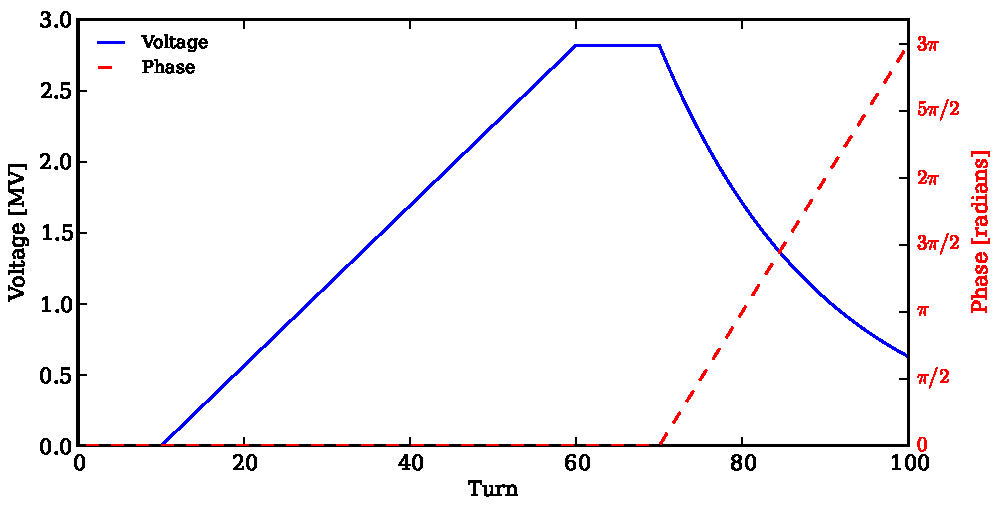
\includegraphics{figures/fail_voltagePhase2v2}
  \caption{Singals generate by \texttt{DYNK} example for ramp + exponential decay of crab voltage\index{crab cavity}\index{crab voltage}, and also linear drift of crab phase. Only the signals for CRAB\_IP1\_L1 are shown. The plot is made from the data in \texttt{dynksets.dat}.}
  \label{fig:DYNK_fail}
\end{figure}

This slightly more complicated example builds on the example given above.
It shows how to change two parameters (voltage and phase) of several objects.
It also demonstrates how functions can be chained together, making more complicated functions.
Some of the resulting functions are shown in Figure~\ref{fig:DYNK_fail}, and the \texttt{DYNK} block here looks like:
\begin{cverbatim}
DYNK
  DEBUG

  FUN zero CONST 0.0
  FUN CV_R1 GET CRAB_IP1_R1 voltage
  FUN CV_R2 GET CRAB_IP1_R2 voltage
  FUN CV_R3 GET CRAB_IP1_R3 voltage
  FUN CV_R4 GET CRAB_IP1_R4 voltage
  FUN CV_L  GET CRAB_IP1_L1 voltage
  FUN ramp LIN 0.02 0
  FUN ramp_R1 MUL CV_R1 ramp
  FUN ramp_R2 MUL CV_R2 ramp
  FUN ramp_R3 MUL CV_R3 ramp
  FUN ramp_R4 MUL CV_R4 ramp
  FUN ramp_L  MUL CV_L  ramp
  SET CRAB_IP1_R1 voltage zero 1 10 0
  SET CRAB_IP1_R2 voltage zero 1 10 0
  SET CRAB_IP1_R3 voltage zero 1 10 0
  SET CRAB_IP1_R4 voltage zero 1 10 0
  SET CRAB_IP1_L1 voltage zero 1 9 0
  SET CRAB_IP1_L2 voltage zero 1 9 0
  SET CRAB_IP1_L3 voltage zero 1 9 0
  SET CRAB_IP1_L4 voltage zero 1 9 0

  SET CRAB_IP1_R1 voltage ramp_R1 11 61 -11
  SET CRAB_IP1_R2 voltage ramp_R2 11 61 -11
  SET CRAB_IP1_R3 voltage ramp_R3 11 61 -11
  SET CRAB_IP1_R4 voltage ramp_R4 11 61 -11
  SET CRAB_IP1_L1 voltage ramp_L 10 60 -10
  SET CRAB_IP1_L2 voltage ramp_L 10 60 -10
  SET CRAB_IP1_L3 voltage ramp_L 10 60 -10
  SET CRAB_IP1_L4 voltage ramp_L 10 60 -10

  ! Voltage decay and detuning
  FUN expCore LIN -0.05 0.0
  FUN decay EXP expCore
  FUN decayScaled MUL decay CV_L
  SET CRAB_IP1_L1 voltage decayScaled 70 100 -70
  SET CRAB_IP1_L2 voltage decayScaled 70 100 -70
  SET CRAB_IP1_L3 voltage decayScaled 70 100 -70
  SET CRAB_IP1_L4 voltage decayScaled 70 100 -70
  FUN phasedrift LIN 0.3141592654 0.0
  SET CRAB_IP1_L1 phase phasedrift 70 100 -70
  SET CRAB_IP1_L2 phase phasedrift 70 100 -70
  SET CRAB_IP1_L3 phase phasedrift 70 100 -70
  SET CRAB_IP1_L4 phase phasedrift 70 100 -70
NEXT
\end{cverbatim}
The first functions defined here are the same as above, storing the default values (as defined in the single element list) for the relevant elements and also zero.
Then follows a normalized linear ramp function \texttt{ramp}, with gradient $0.02 = 1/50$.
This is then used by the ``specialized'' ramp functions \texttt{ramp\_R1$\cdots$R4}, which scales \texttt{ramp} so that the end point is the standard voltages for $t\in 0\ldots50$.

These functions are used to first set the crabs to $0.0$ for the first $9$ revolutions, and in the 10th revolution the ramp starts.
As the \texttt{ramp} function is defined starting at turn $0$, a shift $-10$ or $-11$ is applied to the ramps.
The ramp is switched off after turn 60/61, leaving the crabs to be operating at the last \texttt{SET} value.

Further, we want to demonstrate a failure in the crab voltage\index{crab voltage}.
This is done using an exponential decaying function $V(t) = V_0 \exp\left(-0.05 t\right)$, which is implemented as three chained functions:

\bigskip
\begin{tabular}{@{}lp{0.8\linewidth}}
    \textbf{expCore}     & $f(t) = -0.05 t + 0.0$ \\
    \textbf{decay}       & $g(t) = \exp(f(t)) = \exp(-0.05 t + 0.0)$ \\
    \textbf{decayScaled} & $h(t) = V_0 \cdot g(f(t)) = V_0 \cdot \exp(f(t)) = \exp(-0.05 t + 0.0)$
\end{tabular}

\bigskip
For the \texttt{SET}, the time $t$ is then shifted by $-70$ turns, so that the functions are evaluated starting at $t=0$.

% \paragraph{Detuning a cavity (accelerating or crab)}~\\
% Needs writing!

\paragraph{Using the PIPE function}~\\
%Note: This example is referenced from the FUN table.

To use the \texttt{PIPE} functionality, add a \texttt{FUN} and \texttt{SET} to the \texttt{DYNK} block such as:
\begin{cverbatim}
FUN pipe1 PIPE /tmp/pip1 /tmp/pip2 myID1 4242
SET  ACFCA.AR1.B1 voltage pipe1 10 -1 -9
\end{cverbatim}
Then create the two pipes using the \texttt{mkfifo} UNIX command, e.g.\ \texttt{mkfifo~pip1} and \texttt{mkfifo~pip2} in the chosen directory.
When starting SixTrack, it will first open the input pipe (while reading the \texttt{DYNK} block), and wait for the external program to do the same.
This can be simulated by running \texttt{cat~>~pip1}; it is also possible to open the input pipe before starting SixTrack.
After opening the input pipe, SixTrack will open the output pipe, again this can be simulated by running \texttt{cat~pip2}, and again this pipe may be opened before starting SixTrack.
Note that when SixTrack ends, the output pipe will be closed, so the receiving \texttt{cat} process is terminated.

After opening the output pipe, SixTrack writes the line \texttt{DYNKPIPE~!******************!} to this file.
It then writes a line similar to \texttt{INIT~ID=myID1~for~FUN=pipe1} for each \texttt{FUN} using this output pipe.

During tracking, when one of the \texttt{PIPE} \texttt{FUN}s are called SixTrack writes a line similar to \texttt{GET ID=myID1 TURN=~1} to the output pipe.
Note that the turn number is the one passed to the \texttt{FUN} from \texttt{SET}, i.e. including any turn-shift.
It then waits for a single floating point number to be written (in ascii) to the input pipe, which is then read and returned from the \texttt{FUN}.

% ================================================================================================================================ %
\section{Beam--Beam Element} \label{BeamBeam}

The beam--beam kick, including a separation of the beams, is treated \`{a} la Basetti and Erskine~\cite{BasErs} and implemented as in MAD-X~\cite{MAD}.\index{beam--beam}\index{BEAM}
However, a much faster but nevertheless precise calculation using interpolation can be used~\cite{ERIC}.
Since SixTrack version 3, the beam--beam is also available in the 6D form \`{a} la Hirata~\cite{Hirata}.
Lastly, the linear coupling has been considered in 4 and 6 dimensional phase space~\cite{ripbeam}.

\bigskip
\begin{tabular}{@{}lp{0.8\linewidth}}
    \textbf{Keyword}    & \texttt{BEAM}\index{BEAM} \\
    \textbf{Data lines} & $>1$ \\
    \textbf{Format}     & Two different input formats are available, ``traditional'' and ``EXPERT''. If ``EXPERT'' mode is wanted, this is triggered by adding the flag \texttt{EXPERT}\index{BEAM EXPERT} on the first line of the block.
\end{tabular}

\paragraph{Traditional format}~\\

\bigskip
\begin{tabular}{@{}lp{0.8\linewidth}}
    First line:    & \texttt{partnum emitnx emitny sigz sige ibeco ibtyp lhc ibbc} \\
    Further lines: & \texttt{name ibsix xang xplane xstr}
\end{tabular}

\bigskip
\begin{longtabu}{@{}llp{0.65\linewidth}}
    \texttt{partnum}       & float   & Number of particles in bunch \\
    \texttt{emitnx,emitny} & floats  & Horizontal and vertical normalised emittance\index{normalised emittance} respectively [$\mu \mbox{m}\cdot\mbox{rad}$] \\
    \texttt{sigz,sige}     & floats  & r.m.s. bunch length [m] and r.m.s. energy spread \\
    \texttt{ibeco}         & integer & Switch (0 = off; 1 = on) to subtract the closed orbit introduced by the separation of the beams. It is recommended to always subtract it as it is not yet calculated in a selfconsistent manner. The \texttt{ibeco} switch also acts on the ``wire'' elements \ref{sec:WIRE} in the same way as on the beam-beam elements. It subtracts the closed orbit introduced by the wire if \texttt{ibeco}=1 and applies it if \texttt{ibeco}=0. \\
    \texttt{ibtyp}         & integer & Switch (0 = off; 1 = on) to use the fast beam--beam algorithms developed in collaboration with G.A.~Erskine and E.~McIntosh.  The linear optics are calculated with ``exact'' beam--beam kicks. \\
    \texttt{lhc}           & integer & For the LHC with its anti-symmetric IR the separation of the beams in one plane can be calculated by the $\beta$-function of the other plane. For flat beams (not anti-symmetric optics) the separation can be loaded from the \texttt{fort.2} file. (0 = off; 1 = anti-symmetric; 2 = load from file). \\
    \texttt{ibbc}          & integer & Linear coupling considered in 4D and 6D (0 = off; 1 = on). \\
    \texttt{name}          &           & Name of 6D beam--beam element. Beam--beam elements that do not appear will be treated as 4D kicks. \\
    \texttt{ibsix}         & integer & Number of slices of the 6D beam--beam element. If \texttt{ibsix} is set to 0 this element is treated as a 4D element. \\
    \texttt{xang}          & float   & Half crossing angle\index{half crossing angle} (angle the between the trajectories of the two beams) at this particular element [rad]. \\
    \texttt{xplane}        & float   & Crossing plane angle [rad]. \\
    \texttt{xstr}          & float   & Angle of the position of the slices in the boosted frame [rad] (i.e. $X = Z \sin(\mathit{xstr}) \cos(\mathit{xplane})$, $Y =Z \sin(\mathit{xstr}) \cos(\mathit{xplane})$ ).  In absence of crabbing user should make sure \texttt{xstr=xang}; in case the \texttt{xstr} flag is not set then \texttt{xstr=xang} is assumed and a warning is printed (since version 4.5.45).
\end{longtabu}

\paragraph{EXPERT format}~\\

\bigskip
\begin{longtabu}{@{}lp{0.8\linewidth}}
    First line:   & \texttt{EXPERT}\index{BEAM EXPERT} \\
    Second line:  & \texttt{partnum emitnx emitny sigz sige ibeco ibtyp lhc ibbc} \\
    Further lines & 4D BB lens (1 line per element): \\
                  & ~~~~\texttt{name ibsix $\Sigma_{x,x}$ $\Sigma_{y,y}$ h-sep v-sep strength-ratio $\Sigma_{x,y}$} \\
                  & 6D BB lens (3 lines per element): \\
                  & ~~~~\texttt{name ibsix xang xplane h-sep v-sep} \\
                  & ~~~~\texttt{$\Sigma_{x,x}$ $\Sigma_{x,xp}$ $\Sigma_{xp,xp}$ $\Sigma_{y,y}$ $\Sigma_{y,yp}$} \\
                  & ~~~~\texttt{$\Sigma_{yp,yp}$ $\Sigma_{x,y}$ $\Sigma_{x,py}$ $\Sigma_{xp,y}$ $\Sigma_{xp,yp}$ strength-ratio}
\end{longtabu}

\bigskip
Some parameters are new or defined in a different way:

\bigskip
\begin{longtabu}{@{}llp{0.65\linewidth}}
    \texttt{lhc}   & integer & This parameter is kept for now only for RHIC studies when equal to 9. \\
    \texttt{name}  &         & Name of the beam--beam element. \\
    \texttt{ibsix} & integer & Number of slices of the 6D beam--beam element.\\
                   &         & If \texttt{ibsix} is set to 0, this element is treated as a 4D element.\\
                   &         & If \texttt{ibsix} is larger or equal 1, this element is treated as a 6D element. \\
    $\Sigma_{xx}$  & float   & Horizontal $\sigma$ for the strong beam\index{strong beam} $\rm{[mm^2]}$. \\
    $\Sigma_{yy}$  & float   & Vorizontal $\sigma$ for the strong beam $\rm{[mm^2]}$. \\
    $\Sigma_{xy}$  & float   & Coupled $\sigma$ for the strong beam $\rm{[mm^2]}$. Optional, used only if \texttt{ibbc=1}. \\
    \texttt{h-sep} & float   & Horizontal beam--beam separation\index{beam--beam separation} [mm] \\
    \texttt{v-sep} & float   & Vertical beam--beam separation [mm] \\
    \texttt{strength-ratio} & float & Strength ratio with respect to the nominal beam--beam kick strength\index{beam--beam kick}. This is useful to allow for splitting one beam--beam kick into several (longitudinally close by) kicks.\\
    $\Sigma_{i,j}$ & float   & Second order momenta matrix for the strong beam, in units of mm and mrad. For example $\Sigma_{xxp}$ in [mm\ mrad]
\end{longtabu}

\paragraph{Conversion from traditional to EXPERT format}~\\

An automatic converter from the ``traditional'' input block to the new ``expert'' format is built into SixTrack; every time a non-\texttt{EXPERT} input block is encountered, a conversion is printed to the standard output.
Therefore, all the user needs to do is to run SixTrack (number of turns does not matter) on an input file that should be converted, and follow the instructions which are printed at the beginning of the program output.

\paragraph{Remarks}~\\

These beam--beam elements have to appear in the single element list (\ref{NonEle}) (type 20).
If the ``traditional'' option is used in the \texttt{BEAM} block, the listing in the single element list must contain their horizontal and vertical beam--beam separations (see~\ref{BBS}).

\paragraph{Sign Convention}~\\

Some clarifications regarding the sign convention used for the separation and crossing angle variables.
%\todo[inline]{Check if applies to both ``traditional'' and ``EXPERT'' format.}

\paragraph{Separations:}~\\
\begin{enumerate}
    \item The separation is added to the transverse coordinates of each particles just before the beam-beam subroutines (see Fig.~\ref{fig:BB_sep}).
        \begin{eqnarray*}
            \tilde x_{i} = x_{i} + \mathrm{sep}_{x} - \mathrm{CO}_{x} \\
            \tilde y_{i} = y_{i} + \mathrm{sep}_{y} - \mathrm{CO}_{y}
        \end{eqnarray*}
    \item Lorentz boost\index{Lorentz boost} applied to the updated coordinates.
    \item The separation used for the actual beam-beam kick (sep$_{x,y,kick}$) is the difference between the centroid of the strong slice (X$^{\dag}$,Y$^{\dag}$) and the each particle (x$_i$,y$_i$).
    \item Antiboost to return to accelerator frame.
    \item The separation is removed and the closed orbit is added back. Tracking continues.
        \begin{eqnarray*}
            \tilde x_{i} = x_{i} - \mathrm{sep}_{x} + \mathrm{CO}_{x} \\
            \tilde y_{i} = y_{i} - \mathrm{sep}_{y} + \mathrm{CO}_{y}
        \end{eqnarray*}
\end{enumerate}
\begin{figure}[h]
    \begin{center}
    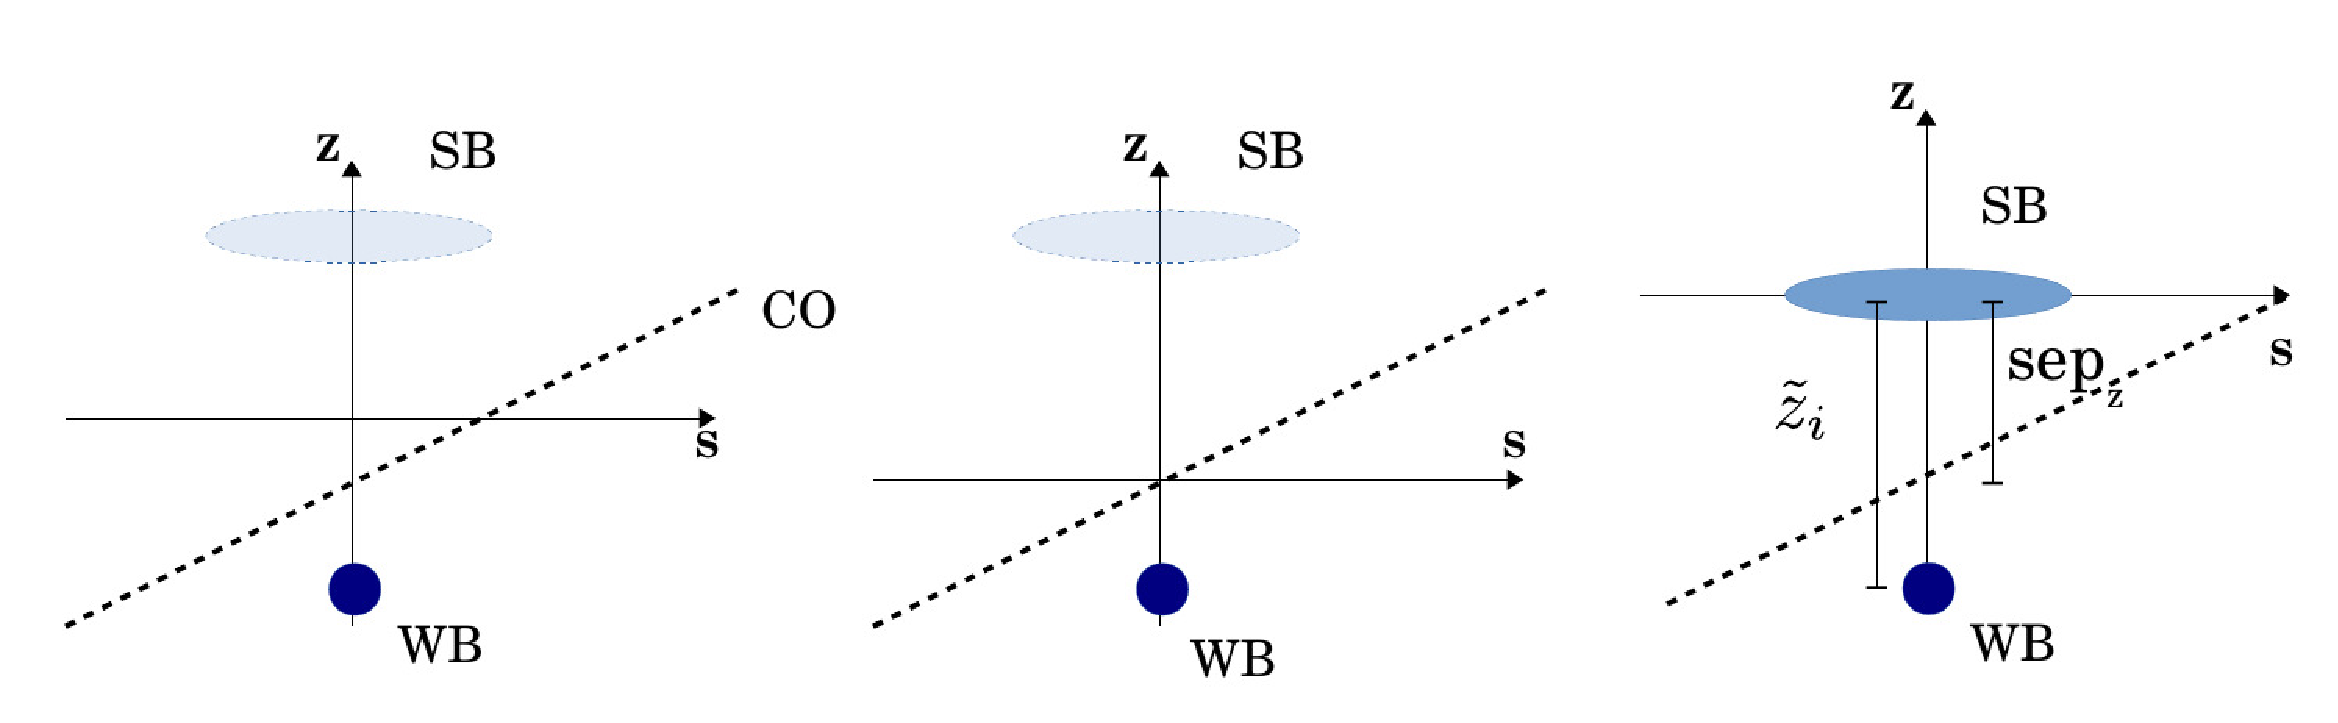
\includegraphics[width=0.8\textwidth]{figures/BB_sep}
    \caption{Coordinate manipulation taking into consideration the beam-beam lens separation as stated in point 1 of the separation sign convention.}
    \label{fig:BB_sep}
    \end{center}
\end{figure}

\paragraph{Crossing angles:}~\\
\begin{enumerate}
    \item The closed orbit\index{closed orbit} is removed just before the beam-beam subroutines.
        \begin{eqnarray*}
            \tilde x^{\prime}_{i} = x^{\prime}_{i} - \mathrm{CO}_{x^{\prime}} \\
            \tilde y^{\prime}_{i} = y^{\prime}_{i} - \mathrm{CO}_{y^{\prime}}
        \end{eqnarray*}
    \item Lorentz boost applied to the updated coordinates.
    \item Apply Synchro-Betatron Mapping\index{synchro-betatron mapping}.
    \item Antiboost to return to accelerator frame.
    \item The closed orbit\index{closed orbit} is added back. Tracking continues.
        \begin{eqnarray*}
            \tilde x^{\prime}_{i} = x^{\prime}_{i} + \mathrm{CO}_{x^{\prime}} \\
            \tilde y^{\prime}_{i} = y^{\prime}_{i} + \mathrm{CO}_{y^{\prime}}
        \end{eqnarray*}
\end{enumerate}
\begin{figure}[h]
    \begin{center}
    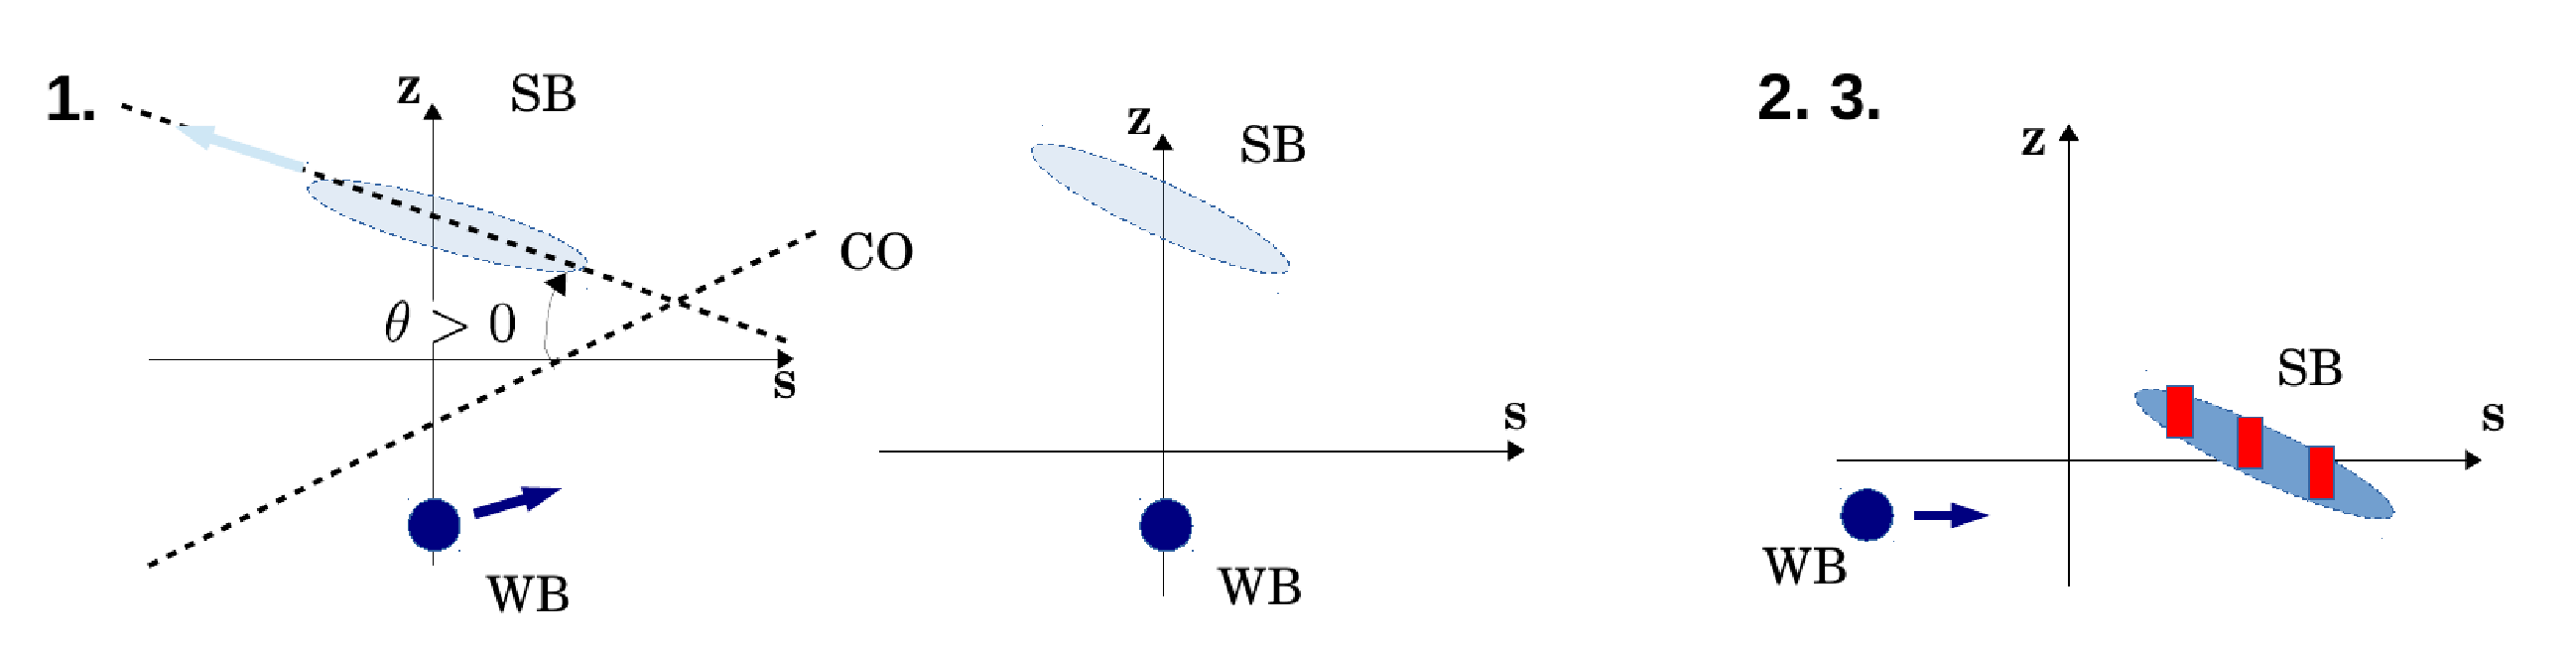
\includegraphics[width=0.8\textwidth]{figures/BB_xsing}
    \caption{Coordinate manipulation to move from the accelerator frame to a head-on collision frame (Figures left and center). A positive crossing angle is considered as shown in the left figure. Then Lorentz boost and Synchro-Betatron Mapping are applied (right).}
    \label{fig:BB_xsing}
    \end{center}
\end{figure}

% ================================================================================================================================ %
\section{Wire} \label{sec:WIRE}

The wire block serves for reading in the input parameters for the wire.\index{WIRE}
Each wire also needs to be added as single element in the list of single elements.

\bigskip
\begin{tabular}{@{}lp{0.8\linewidth}}
    \textbf{Keyword}    & \texttt{WIRE}\index{WIRE} \\
    \textbf{Data lines} & Variable \\
    \textbf{Format}     & \texttt{name flag\_co current int\_length phys\_length disp\_x disp\_y tilt\_x tilt\_y} \\
                        & A description of the input parameters for the wire is given in Table~\ref{tab:wire}.
\end{tabular}

\begin{center}
\begin{longtable}{|p{2.0cm} |p{1.4cm} |p{9.2cm}|}
    %Note: \\* (with the star) used to inhibit page breaks in the middle of groups of the same type
    \caption{Input parameters for the \texttt{WIRE} block.}
    \label{tab:wire} \\*
    \hline
    \rowcolor{blue!30}
    Arguments & Unit & Description \\*
    \hline
    \endfirsthead

    \hline
    \rowcolor{blue!30}
    Arguments & Unit & Description \\*
    %\hline
    \endhead

    \rowcolor{gray!15}
    \multicolumn{3}{|c|}{(The table continues on the next page)}\\*
    \hline
    \endfoot

    \hline
    \endlastfoot

    \hline

    \texttt{name} & - &
    Name of wire. Must be the same as in list of single elements\index{single elements}.\\*
    \hline

    \texttt{flag\_co} & - &
    flag to define the displacement of the wire in respect to the closed orbit\index{closed orbit} or x=y=0. For \texttt{flag\_co}=+1 \texttt{disp\_*} is the distance between x=y=0 and the wire. For \texttt{flag\_co}=-1 \texttt{disp\_*} is the distance between the closed orbit and the wire.\\*
    \hline

    \texttt{current} & A &
    wire current\index{wire current} \\*
    \hline

    \texttt{int\_length} & m &
    integrated length of the wire\\*
    \hline

    \texttt{phys\_length} & m &
    physical length of the wire\\*
    \hline

    \texttt{disp\_x} & mm &
    hor. displacement of the wire\\*
    \hline

    \texttt{disp\_y} & mm &
    vert. displacement of the wire\\*
    \hline

    \texttt{tilt\_x} & degrees &
    hor. tilt of the wire\index{wire tilt} $-90 < tilt\_x < 90$ (uses same defintion as DISP block) \\*
    \hline

    \texttt{tilt\_y} & degrees &
    vert. tilt of the wire $-90 < tilt\_y < 90$ (uses same defintion as DISP block) \\*
    \hline
\end{longtable}
\end{center}

\paragraph{Remarks}~\\

The user has to check that the wires defined in the WIRE block are also defined in the list of single elements and vice versa.
All parameters, except for the type (type 15), are ignored in the single element definition and the execution is aborted if the parameters are non-zero.
In addition to the parameters defined in the \texttt{WIRE} block, the \texttt{ibeco} parameter in the \texttt{BEAM} block (see Section~\ref{BeamBeam}) imposes the same behavior on the wire as for beam-beam.
Explicitly, the closed orbit introduced by the wire is subtracted if \texttt{ibeco}=1 and not subtracted if \texttt{ibeco}=0.

\paragraph{Example:}~\\

In the following we give some examples for wire definitions.
This example defines two wires \texttt{wire\_1} and \texttt{wire\_2}.

The input block in \texttt{fort.3} is given by:
\begin{cverbatim}
WIRE
wire_1   -1  +98.9   2.0  1.0   10.0   10.0     1.1     1.1
wire_2   -1  +98.9   2.0  1.0   10.0   10.0     0.0     0.0
NEXT
\end{cverbatim}
The single and structure element definition in \texttt{fort.2} is given by:
\begin{ctverbatim}
SINGLE ELEMENTS---------------------------------------------------------
...
wire_1   15 0.000000000e+00 0.000000000e+00  0.000000000e+00  0.000000000e+00  0.000000000e+00  0.000000000e+00
wire_2   15 0.000000000e+00 0.000000000e+00  0.000000000e+00  0.000000000e+00  0.000000000e+00  0.000000000e+00
...
STRUCTURE INPUT---------------------------------------------------------
...
BLOC56            wire_1              wire_2
...
\end{ctverbatim}
Note that all parameters except for the type have to be set to 0 in the single element definition.

% ================================================================================================================================ %
\section{``Phase Trombone'' Element} \label{Trombone}

The linear ``phase trombone'' allows for the introduction of an arbitrary transfer matrix.\index{phase trombone}\index{TROM}
It can be used to introduce a change in the transverse phases without spoiling the linear optics of the rest of the machine, i.e. the Twiss parameters are the same at entrance and exit of the element.
Note that it is up to the user to construct the matrix. The coordinates used as inputs are: $x$, $p_x$, $y$ ,$p_y$, $\sigma$, $p_{\sigma}$.

\bigskip
\begin{tabular}{@{}lp{0.8\linewidth}}
    \textbf{Keyword}    & \texttt{TROM}\index{TROM} \\
    \textbf{Data lines} & 1 line with name and then in blocks of 14 lines with 3 entries each. \\
    \textbf{Format}     & First line: \texttt{name} \\
                        & Second line:  $x$, $p_x$, $y$ \\
                        & Third line:  $p_y$, $\sigma$, $p_{\sigma}$ \\
                        & Fourth util $15^{th}$: \texttt{M($ 6 \times 6$)} matrix
\end{tabular}

\bigskip
\begin{tabular}{@{}llp{0.6\linewidth}}
    \texttt{name} & char & May contain up to 48 characters. \\
    \texttt{cx, cx', cy, cy', cz, cz'} & floats & 6D closed orbit\index{closed orbit} to be added to the coordinates. \\
    \texttt{M($ 6 \times 6$)} & floats & $ 6 \times 6$ matrix elements.
\end{tabular}

\paragraph{Remarks}~\\

The user has to make sure that the above stated conditions are fulfilled.
When using the $mad\_6t$~\cite{CONVERTOR} converter from MAD-X\index{MAD-X} to SixTrack, this is guaranteed to be the case.
Note also that the crossterms between the transverse plains are not considered for the time being.

% ================================================================================================================================ %
\section{Beam Distribution EXchange (BDEX)} \label{sec:BDEX}

The Beam Distribution EXchange allows an external program to read and modify the beam distribution in SixTrack.\index{BDEX}
This can be used for tracking part of the machine in an external program, for example for including physics processes that are normally not available in SixTrack.
Another possible use is for multi-bunch tracking, i.e.\ with an external program ``swapping'' the bunch at a some point in the ring.
This would be useful for studying (for example) beam loading, where the external program would read the position of a bunch in the cavity, use that to compute an update of the cavity voltage (which can be sent to SixTrack using DYNK FUN PIPE), swap the bunch with another one and track that to the cavity (still at ``physics turn'' 1, but ``SixTrack turn'' 2) etc.

Please note that \texttt{BDEX} is currently not supported in the checkpoint/restart\index{checkpoint/restart} version or in the collimation\index{collimation} version.
Including \texttt{BDEX} in one of these versions results in a run-time error.

\bigskip
\begin{tabular}{@{}lp{0.8\linewidth}}
    \textbf{Keyword}    & \texttt{BDEX}\index{BDEX} \\
    \textbf{Data lines} & Variable \\
    \textbf{Format}     & There are three types of statements possible in a \texttt{BDEX} block, listed below.
\end{tabular}

\bigskip

\paragraph{ELEM} \texttt{ELEM chanName elemName action}\\

This associates a given element with an already existing channel and an action.
The element must appear in the SINGLE ELEMENT\index{single elements} block, and be of type 0 (marker).
The action indicates what should be done with the particle distribution when it reaches this element.
Currently, the only allowed action is ``1'', which means ``particle exchange'', i.e.\ output the beam distribution and read back another one at the same point.

\paragraph{CHAN} \texttt{CHAN chanName chanType \ldots}\\

This creates a new channel through which the \texttt{BDEX} can communicate.
Currently, the only implemented \texttt{chanType} is \texttt{PIPE}, however \texttt{TCPIP} is also foreseen.

For the \texttt{PIPE} type, the statement including arguments is \texttt{CHAN PIPE inPipeName outPipeName format fileUnit}.
This uses a pair of UNIX FIFOs, through which SixTrack can communicate with an external program.
When the channel is used, it sends a message on the outpipe, then waits for a reply with the new distribution over the inPipe.
The \texttt{format} is an integer used to indicate the output/input format, and is currently unused.
The \texttt{fileUnit} is the Fortran unit number that should be used to open the inPipe.
The \texttt{outPipe} is opened on the next unit, so both units fileUnit and fileUnit+1 must be free.

\paragraph{DEBU}~\\

This statement switches on extra ``debugging'' output from \texttt{BDEX}\index{DEBUG}.
This can be useful if debugging the code or if debugging the input.

\subsection{Communication protocols}

The communication protocols used by the different channel types are listed below:

\paragraph{PIPE communication protocol}~\\

When a pair of pipes are first initialized, a header ``\texttt{BDEX-PIPE !******************!}'' is written to the output pipe.
Then, when the tracking reaches an element which is marked as active for this channel, it writes another header like ``\texttt{BDEX TURN= 1 BEZ=ip1 I= 1 NAPX= 64}'', where \texttt{TURN} is the number of the current SixTrack turn, \texttt{BEZ} the name of the SINGLE ELEMENT, \texttt{I} the index of the STRUCTURE ELEMENT, and \texttt{NAPX} the number of particles to be written out.
After this follows \texttt{NAPX} lines with the particle information (one per particle), each line of the format \texttt{xv(1,j) yv(1,j) xv(2,j) yv(2,j) sigmv(j) ejv(j) ejfv(j) rvv(j) dpsv(j) oidpsv(j) dpsv1(j),nlostp(j)} where all but the last floating point numbers, the last being an integer.
Finally, it writes ``\texttt{BDEX WAITING...}'' to the output pipe, and waits for data on the input pipe.

The first line expected on the input pipe should be an integer containing the number of particles to write back.
If this integer is -1, the current particle distribution is kept.
Otherwise, a number of lines of the same format as with the output is expected.
After reading in the expected number of particles, the string ``\texttt{BDEX TRACKING...}'' is written to the output pipe and tracking is resumed.

\paragraph{TCPIP communication protocol}~\\

TCPIP is not yet implemented, as it would require an external library.
The FLUKA version implements this, we should make sure that we are compatible with their requirements and ideally their protocol.

% ================================================================================================================================ %
\section{Electron Lens} \label{sec:elen}

The electron lens module serves for reading in the input parameters of electron lenses.\index{electron lens}\index{ELENS}
Each e-lens also needs to be added as single element in the list of single elements.
Currently, the ideal electron lens is implemented, i.e.
\begin{itemize}
\item an ideal e--beam distribution, i.e.~no errors (or asymmetries), and all electrons travel parallel to the e-lens axis;
\item the kick is only due to the transverse components of the electric and magnetic fields generated by the electron beam.
  Hence, no longitudinal component of the kick is considered and no energy update is performed.
\end{itemize}

\bigskip
\begin{tabular}{@{}lp{0.8\linewidth}}
    \textbf{Keyword}    & \texttt{ELEN}\index{ELEN} \\
    \textbf{Data lines} & Variable \\
    \textbf{Format}     & There are different types of statements possible in a \texttt{ELEN} block, listed in the following subsections. \\
\end{tabular}

\bigskip
\noindent All the electron lenses are by default considered for calculation by FOX. Nevertheless, the e-lens kick is actually taken into account in the FOX part only if the closed orbit falls in the region of the electron beam or outside, i.e.~no FOX calculation is performed in the hollow part. The user can specify in the \texttt{fort.3} if each e-lens should be considered or not in the FOX calculation (see Sec.~\ref{sec:elen:FOX}).

\noindent It should be noted that by default electrons are considered as beam of the e-lens.
The user is also given the possibility to change the species of the beam of the e-lens to anything they want via the \texttt{SPEC} statement (see Sec.~\ref{sec:elen:SPEC}).
In the following, the description refers to an electron beam, but all the statements also hold for any species requested by the user.

\subsection{Declaration of a lens}\label{sec:elen:declaration}
\begin{tabular}{@{}lp{0.8\linewidth}}
    \textbf{Format}     & \texttt{name type theta\_r2 r2 r1 offset\_x offset\_y (L I E\_k) } \\
    & The last three parameters are optional, but if specified, all of them must be present; they force the re-computation of the angle at \texttt{r2} \texttt{theta\_r2}, taking into account also the beam energy.  \\
    & Additional parameters specific to the electron distributions (see later) must be specified before the optional ones. \\
\end{tabular}

\bigskip
\noindent Currently, four types of electron beam profiles on the transverse plane (i.e.~in the $xy$-plane) are supported:

\bigskip
\begin{tabular}{@{}lp{0.8\linewidth}}
    \texttt{UNIFORM}  & e--beam with constant density of electrons. \\
    \texttt{GAUSSIAN} & e--beam with a radial Gaussian profile. \\
    \texttt{RADIAL}   & e--beam follows a radial distribution as described in a plain ASCII file. \\
    \texttt{WIRE}     & degenerate case of e-lens to a wire, i.e. the beam is concentrated in only one point. \\
\end{tabular}

\begin{center}
\begin{longtable}{| p{2.4cm} | p{1.0cm} | p{12.0cm}|}
    %Note: \\* (with the star) used to inhibit page breaks in the middle of groups of the same type
    \caption{Input parameters for the \texttt{ELEN} block.}
    \label{tab:elen} \\*
    \hline
    \rowcolor{blue!30}
    Argument & Unit & Description \\*
    \hline
    \endfirsthead

    \hline
    \rowcolor{blue!30}
    Argument & Unit & Description \\*
    %\hline
    \endhead

    \rowcolor{gray!15}
    \multicolumn{3}{|c|}{(The table continues on the next page)}\\*
    \hline
    \endfoot

    \hline
    \endlastfoot

    \hline
    \rowcolor{blue!15}
    \multicolumn{3}{|l|}{Valid for all types} \\*

    \texttt{name} & -- & Name of e-lens. Must be the same as that in the list of single elements\index{single elements}.\\*
    \hline

    \texttt{type} & -- & Type of e-lens - either \texttt{UNIFORM}, \texttt{GAUSSIAN}, \texttt{RADIAL}, or \texttt{WIRE}. \\*
    \hline

    \texttt{theta\_r2} & mrad & Kick\footnote{Total, \emph{not} per charge.} received at $r=r_2$ where $r_2$ is the outer radius of the e-lens.
    If negative (negative charge of e-lens beam, see Sec.~\ref{sec:elen:SPEC}), the kick is radially inwards; conversely, if positive, the kick is radially outwards. \\*
    \hline

    \texttt{r2} & mm & Outer radius of the e-lens.\\*
    \hline

    \texttt{r1} & mm & Inner radius of the e-lens. \\* % Can be 0 but not negative.\\*
    \hline

    \texttt{offset\_x} & mm & Horizontal offset of the e-lens.\\*
    \hline

    \texttt{offset\_y} & mm & Vertical offset of the e-lens.\\*
    \hline

    \hline
    \rowcolor{blue!15}
    \multicolumn{3}{|l|}{Specific to \texttt{GAUSSIAN} type} \\*

    \texttt{sig\_el} & mm & $\sigma$ of the electron beam.\\*
    \hline

    \rowcolor{blue!15}
    \multicolumn{3}{|l|}{Specific to \texttt{RADIAL} type} \\*

    \texttt{filename} & & filename of the radial profile. Please see Sec.~\ref{sec:elen_rad_prof} for proper formatting of the file. The profile is read from the file, radially integrated and normalised to the total current. Hence, the kick at \texttt{r2} is given by the value of \texttt{theta\_r2} (or by the optional parameters) and not by integration of the radial profile. The kick is obtained interpolating the normalised profile (see Sec.~\ref{sec:elen:INTER}). The domain of the profile must be larger than the domain identified by \texttt{r1} and \texttt{r2}. \\*
    \hline

    \hline
    \rowcolor{blue!15}
    \multicolumn{3}{|l|}{Optional arguments (all types)} \\*

    \texttt{L} & m & Length of the e-lens. Must be positive. \\*
    \hline

    \texttt{I} & A & Electron current of the e-lens. Must be non--zero. A positive current corresponds to a positive charge flowing in the same direction as that of the main beam. \\*
    \hline

    \texttt{E\_k} & keV & kinetic energy of electrons in the e-lens. Must be positive.\\*
    \hline

\end{longtable}
\end{center}

\bigskip
\paragraph{Remarks}~\\

\begin{enumerate}
\item The spatial charge density of all profiles is defined between \texttt{r1} and \texttt{r2}:
\begin{equation}
  \rho(r)=\left\{
    \begin{array}{ll}
        0 & \mbox{if $r < r_1$} \\
        f(r) & \mbox{if $r_1 \le r < r_2$} \\
        0 & \mbox{if $r_2 \le r$} \\
    \end{array}
    \right. \\
\end{equation}
Moreover, if $r_1=0$, then the lens is full; otherwise, it is hollow.

\item The user has to check that the e-lens defined in the \texttt{ELEN} block is also defined in the list of single elements and vice versa.
  All parameters in the single element definition except the type (type \texttt{29}) are ignored.
\item The current implementation (ideal e-lenses) has no explicit energy--dependency, except for the user defined parameter \texttt{theta\_r2} (see \cite{sixphys}), in case the user specifies \texttt{L}, \texttt{E\_k} and \texttt{I}.
  In fact, in this case, \texttt{theta\_r2} is re-calculated after input parsing, taking into account the beam energy.
  This parameter is re-computed also during energy ramping by the \texttt{DYNK} module.
\item The implementation is fully chromatic and hence compatible with ion tracking and tracking of species different from the synchronous one only if the three main optional parameters (i.e.\ length, kinetic energy of electrons and current) are specified by the user.
  In fact, only in this case, the code knows the value of the normalised relativistic speed $\beta$ of the beam of the lens;
\item In case of energy ramping, if not \texttt{DYNK}-ed, the kick stays constant, as if the e-lens was ramped in beam current in synch with the rest of the machine.
  On the contrary, if the user specifies the three main optional parameters (i.e.~length, kinetic energy of electrons and current), if not \texttt{DYNK}-ed, the kick is recomputed at any update of the reference energy, as if the e-lens was not ramped.
  Hence, it is responsibility of the user to define the way the e-lens is ramped with beam energy.
\item Note that if the user specifies \texttt{theta\_r2} with DYNK, then, starting with the first turn where it is set via \texttt{DYNK}, \texttt{theta\_r2} is no longer ramped with the energy, as if the e-lens was specified using only this parameter in \texttt{fort.3}.
  However note that the chromatic behaviour, which requires \texttt{E\_k}, is still handled in a physically correct way.
\item When dealing with a radial profile from a plain ASCII file (see Sec.~\ref{sec:elen_rad_prof}), the code checks beforehand that the values of \texttt{r1} and \texttt{r2} specified in the \texttt{fort.3} fall inside the range covered by the map, otherwise the code errors and exits. This is done to avoid wrong extrapolations based on noisy maps.
\item The user can specify \texttt{r1}, \texttt{r2} and \texttt{sig\_el} (the last one only for the \texttt{GAUSSIAN} e-lens) in normalised units, i.e.~in units of betatron $\sigma$ or of momentum cut; the user should specify the normalised emittance in the former case (see Sec.~\ref{sec:elen:EMIN}), or the rms of the delta distribution for the latter (see Sec.~\ref{sec:elen:SIGDPP}). SixTrack will compute the linear optics and then pick up the values at the e-lens to set the three parameters. Please note that, due to the cylindrical symmetry of the implemented e-lens, only one optics function is considered (among the orizontal or vertical plane); moreover, it does not matter how many parameters of an e-lens the user decides to express in normalised units, nevertheless they must all be referred to the same normalised emittance or rms of delta distribution.
\item Computing the optics based on FOX calculations and considering the e-lens for FOX calculations clashes with the possibility of expressing the parameters in normalised units; the reason is that the e-lens calculation in the FOX framework requires \texttt{r1}, \texttt{r2} and \texttt{sig\_el} (the last one only for the \texttt{GAUSSIAN} e-lens) expressed in mm, whereas FOX is run before calculating the optics. Please use \texttt{ilin} set to 1 (see Sec.~\ref{LinOpt}).
\item In case the user requests the \texttt{WIRE} beam distribution, \texttt{r2} keeps the meaning of the position at which the kick reaches the value of \texttt{theta\_r2}, whereas it loses completely the geometrical meaning.
Similarly, the user must set \texttt{r1} to 0 -- if not done by the user, the code will take care of that.
The user has also the possibility to make any of the other distributions become a \texttt{WIRE} one setting \texttt{r1} and \texttt{r2} equal to 0.
In this case, the value of \texttt{theta\_r2} will be reached at r=1~mm.

\end{enumerate}

\subsection{EMIN statement}\label{sec:elen:EMIN}
Similarly to done by the \texttt{SIGDPP} statement (see Sec.~\ref{sec:elen:SIGDPP}), the \texttt{EMIN} line allows the user to declare the normalised emittance and which $\beta$ function should be used in conjunction with the declaration of \texttt{r1}, \texttt{r2} and \texttt{sig\_el} (the last one only for the \texttt{GAUSSIAN} e-lens) in terms of normalised amplitude. By default, the statement applies to the e-lens just declared, but its validity can also be extended to other e-lenses in the \texttt{ELEN} block (e.g.~to avoid repeating the same line for all e-lenses).

\bigskip
\begin{tabular}{@{}lp{0.8\linewidth}}
    \textbf{Format}     & \texttt{EMIN emin (min|max|ave|qve|geo) (ALL|BEF(ORE)|AFT(ER))} \\
    & The last two parameters are optional.  \\
\end{tabular}

\begin{center}
\begin{longtable}{| p{2.4cm} | p{1.0cm} | p{12.0cm}|}
    %Note: \\* (with the star) used to inhibit page breaks in the middle of groups of the same type
    \caption{Input parameters for the \texttt{EMIN} keyword in the \texttt{ELEN} block.}
    \label{tab:elen:EMIN} \\*
    \hline
    \rowcolor{blue!30}
    Argument & Unit & Description \\*
    \hline
    \endfirsthead

    \hline
    \rowcolor{blue!30}
    Argument & Unit & Description \\*
    %\hline
    \endhead

    \rowcolor{gray!15}
    \multicolumn{3}{|c|}{(The table continues on the next page)}\\*
    \hline
    \endfoot

    \hline
    \endlastfoot

    \texttt{emin} & m & normalised emittance.\\*
    \hline

    \texttt{iSet} & -- & Which $\beta$ function should be used:    \\*
    & & \begin{tabular}{@{}lp{0.8\linewidth}}
          \texttt{min}     & minimum among $\beta_x$ and $\beta_y$; \\
          \texttt{max}     & maximum among $\beta_x$ and $\beta_y$; \\
          \texttt{ave}     & algebraic average, i.e.~$\beta=\frac{\beta_x+\beta_y}{2}$; \\
          \texttt{qve}     & quadratic average, i.e.~$\beta=\sqrt{\frac{\beta_x^2+\beta_y^2}{2}}$; \\
          \texttt{geo}     & geometric average, i.e.~$\beta=\sqrt{\beta_x\beta_y}$; \\
        \end{tabular}
    \\*
    & & \texttt{min} is the default.\\*
    \hline
    
    & -- & The stated normalised emittance should be applied also to other e-lenses: \\*
    & & \begin{tabular}{@{}lp{0.8\linewidth}}
      \texttt{ALL}     & all e-lenses being declared; \\
      \texttt{BEF}     & all e-lenses declared before the current one; \\
      \texttt{AFT}     & all e-lenses declared after the current one; \\
    \end{tabular}
    \\*
    & & The default behaviour is that the current \texttt{EMIN} line applies only to the e-lens being declared, without touching the others. \\*
    \hline

\end{longtable}
\end{center}

\bigskip
\noindent It should be noted that, in case the same e-lens (SINGLE ELEMENT) appears many times in the lattice structure, the values of the $\beta$ functions at all the instances of the same e-lens are used, following the algorithm selected by the user.

\subsection{FOX statement}\label{sec:elen:FOX}
The user can modify the default behaviour of SixTrack in considering the kick from electron lenses in the FOX calculation. By default, the statement applies to the e-lens just declared, but its validity can also be extended to other e-lenses in the \texttt{ELEN} block (e.g.~to avoid repeating the same line for all e-lenses).

\bigskip
\begin{tabular}{@{}lp{0.8\linewidth}}
    \textbf{Format}     & \texttt{FOX true|false|on|off (ALL|BEF(ORE)|AFT(ER))} \\
\end{tabular}

\bigskip
\noindent For the last parameter, please see Tab.~\ref{tab:elen:EMIN} in Sec.~\ref{sec:elen:EMIN}, since the same interface is used.

\subsection{INTER statement}\label{sec:elen:INTER}
The user can choose to interpolate the radial profile from a file (see Sec.~\ref{sec:elen_rad_prof}) not linearly but with a polynomial of higher order, up to 19, chosing the number of points to be used for the interpolation. The default is linear interpolation, i.e.~using 2 points. When approaching r=0, the code will force the interpolation with 3 points, in order to match the computed tune-shift to that of a uniform distribution (a sort of linearisation of the kick). By default, the statement applies to the e-lens just declared, but its validity can also be extended to other e-lenses in the \texttt{ELEN} block (e.g.~to avoid repeating the same line for all e-lenses).

\bigskip
\begin{tabular}{@{}lp{0.8\linewidth}}
    \textbf{Format}     & \texttt{INTER elens\_radial\_mpoints (ALL|BEF(ORE)|AFT(ER))} \\
\end{tabular}

\bigskip
\noindent For the last parameter, please see Tab.~\ref{tab:elen:EMIN} in Sec.~\ref{sec:elen:EMIN}, since the same interface is used.

\subsection{SIGDPP statement}\label{sec:elen:SIGDPP}
Similarly to what done by the \texttt{EMIN} statement (see Sec.~\ref{sec:elen:EMIN}), the \texttt{SIGDPP} line allows the user to declare the rms of the delta distribution and which dispersion function should be used in conjunction with the declaration of \texttt{r1}, \texttt{r2} and \texttt{sig\_el} (the last one only for the \texttt{GAUSSIAN} e-lens) in terms of normalised amplitude. By default, the statement applies to the e-lens just declared, but its validity can also be extended to other e-lenses in the \texttt{ELEN} block (e.g.~to avoid repeating the same line for all e-lenses).

\bigskip
\begin{tabular}{@{}lp{0.8\linewidth}}
    \textbf{Format}     & \texttt{SIGDPP sigdpp (min|max|ave|qve|geo) (ALL|BEF(ORE)|AFT(ER))} \\
    & The last two parameters are optional.  \\
\end{tabular}

\begin{center}
\begin{longtable}{| p{2.4cm} | p{1.0cm} | p{12.0cm}|}
    %Note: \\* (with the star) used to inhibit page breaks in the middle of groups of the same type
    \caption{Input parameters for the \texttt{SIGDPP} keyword in the \texttt{ELEN} block.}
    \label{tab:elen:SIGDPP} \\*
    \hline
    \rowcolor{blue!30}
    Argument & Unit & Description \\*
    \hline
    \endfirsthead

    \hline
    \rowcolor{blue!30}
    Argument & Unit & Description \\*
    %\hline
    \endhead

    \rowcolor{gray!15}
    \multicolumn{3}{|c|}{(The table continues on the next page)}\\*
    \hline
    \endfoot

    \hline
    \endlastfoot

    \texttt{sigdpp} & -- & rms of the delta distribution of the beam.\\*
    \hline

    \texttt{iSet} & -- & Which dispersion function should be used:    \\*
    & & \begin{tabular}{@{}lp{0.8\linewidth}}
          \texttt{min}     & minimum among $D_x$ and $D_y$; \\
          \texttt{max}     & maximum among $D_x$ and $D_y$; \\
          \texttt{ave}     & algebraic average, i.e.~$D=\frac{D_x+D_y}{2}$; \\
          \texttt{qve}     & quadratic average, i.e.~$D=\sqrt{\frac{D_x^2+D_y^2}{2}}$; \\
          \texttt{geo}     & geometric average, i.e.~$D=\sqrt{D_xD_y}$; \\
        \end{tabular}
    \\*
    & & \texttt{min} is the default. \\*
    \hline
    
    & -- & For the last parameter, please see Tab.~\ref{tab:elen:EMIN} in Sec.~\ref{sec:elen:EMIN}, since the same interface is used. \\*
    \hline

\end{longtable}
\end{center}

\bigskip
\noindent It should be noted that, in case the same e-lens (SINGLE ELEMENT) appears many times in the lattice structure, the values of the dispersion functions at all the instances of the same e-lens are used, following the algorithm selected by the user.

\subsection{SPEC statement}\label{sec:elen:SPEC}
The \texttt{SPEC} line allows the user to set the species of the beam in the lens to anything they desire.
The default is electrons.
The user can assign only one species to each e-lens, but all e-lenses can have different species.
By default, the statement applies to the e-lens just declared, but its validity can also be extended to other e-lenses in the \texttt{ELEN} block (e.g.~to avoid repeating the same line for all e-lenses).
The species is actually taken into account only if the kick of the lens is calculated internally by the code (see Sec.~\ref{sec:elen:declaration}).
It should be noted that, if the charge is negative, the kick is radially inwards; conversely, if the charge is positive, the kick is radially outwards.

\bigskip
\begin{tabular}{@{}lp{0.8\linewidth}}
    \textbf{Format}     & \texttt{SPEC  m[MeV/c2]  Q[e] (ALL|BEF(ORE)|AFT(ER))} \\
    & The last parameter is optional.  \\
\end{tabular}

\begin{center}
\begin{longtable}{| p{2.4cm} | p{1.2cm} | p{11.8cm}|}
    %Note: \\* (with the star) used to inhibit page breaks in the middle of groups of the same type
    \caption{Input parameters for the \texttt{SPEC} keyword in the \texttt{ELEN} block.}
    \label{tab:elen:SPEC} \\*
    \hline
    \rowcolor{blue!30}
    Argument & Unit & Description \\*
    \hline
    \endfirsthead

    \hline
    \rowcolor{blue!30}
    Argument & Unit & Description \\*
    %\hline
    \endhead

    \rowcolor{gray!15}
    \multicolumn{3}{|c|}{(The table continues on the next page)}\\*
    \hline
    \endfoot

    \hline
    \endlastfoot

    \texttt{m} & MeV/c$^2$ & mass of the species of the beam in the e-lens. \\*
    \hline

    \texttt{Q} & e & charge of the species of the beam in the e-lens. \\*
    \hline

    & -- & For the last parameter, please see Tab.~\ref{tab:elen:EMIN} in Sec.~\ref{sec:elen:EMIN}, since the same interface is used. \\*
    \hline

\end{longtable}
\end{center}

\subsection{Example} \label{sec:elen:example}

In the following we give an example of e-lens definition.
The example defines four electron lenses, i.e.~\texttt{hel1}, \texttt{hel2}, \texttt{hel3} and \texttt{hel4}; the first and fourth ones have a uniform electron density, whereas the second one has an electron beam with a Gaussian profile with $\sigma$=1.1547~mm and the third one makes use of an ASCII file for the radial distribution.
While the first, third and fourth e-lenses are hollow, the second one is full.
For the second and fourth e-lens the user requests the re-computation of the kick, given the length of the lens of 4~m, the electron current of 2~A (opposite wrt the main beam) and the electron kinetic energy of 1~keV, while for all the others kick at \texttt{r2} has been explicitly declares.
The first e-lens is discarded for FOX calculation.
When using the radial profile, interpolation is performed with 4 points, i.e.~using a third order polynomial.
For all e-lenses, in case normalised units are used (which is the case for \texttt{r2} of the second e-lens), a normalised emittance of 3.5~$\mu$m and the minimum among the $\beta$ functions (horizontal and vertical) is used to compute the local beam $\sigma$. The exception is the fourth e-lens, for which \texttt{r1} and \texttt{r2} are given as cut in momentum, using the quadratic average among $D_x$ and $D_y$.
All e-lenses have beams of electrons but the last one, where positrons are used; hence, all the kicks are inwards (due to the negative charge of the electrons) but the last one (redundant, as the kick is re-computed internally by SixTrack).
Please note the change of sign in the current, to keep the beam of both lenses always anti-parallel to the main beam.
The input block in \texttt{fort.3} is then given by:

\begin{cverbatim}
ELEN
EMIN 3.5E-06 min all  
hel1 UNIFORM  -4.920e-03 6.928 4.619 1.1547 2.3093
FOX false
hel2 GAUSSIAN -4.920e-03 -6.0 0.0 1.1547 2.3093 1.1547 4 2 1
hel3 RADIAL   -4.920e-03 5.7735 13.8564  -4.6188  4.6188  my_radial_profile.txt
INTER 4
hel4 UNIFORM   4.920e-03 -5.0 -10.0  -4.6188  4.6188 4 -2 1
SIGDPP 2.8E-03 qve
SPEC 0.510998902  1.0 after
NEXT
\end{cverbatim}
The single and structure element definition in \texttt{fort.2} are given by:
\begin{ctverbatim}
SINGLE ELEMENTS---------------------------------------------------------
...
hel1            29  0.000000000e+00  0.000000000e+00  0.000000000e+00  0.000000000e+00  0.000000000e+00  0.000000000e+00
hel2            29  0.000000000e+00  0.000000000e+00  0.000000000e+00  0.000000000e+00  0.000000000e+00  0.000000000e+00
hel3            29  0.000000000e+00  0.000000000e+00  0.000000000e+00  0.000000000e+00  0.000000000e+00  0.000000000e+00
hel4            29  0.000000000e+00  0.000000000e+00  0.000000000e+00  0.000000000e+00  0.000000000e+00  0.000000000e+00
...
STRUCTURE INPUT---------------------------------------------------------
...
BLOC56            hel1              hel2              hel3              hel4
...
\end{ctverbatim}

\bigskip
\noindent \textbf{Note:} All parameters except for the type are set to \texttt{0} in the single element definition.

\subsection{Format of Radial Profile} \label{sec:elen_rad_prof}
The file format of the radial profile is

\bigskip
\begin{tabular}{@{}lp{0.8\linewidth}}
    \textbf{Data lines} & Variable \\
    \textbf{Comment character} & \texttt{\#} (only as first char of the line) \\
    \textbf{Format}     & \texttt{R} (mm) \texttt{J} (A cm$^{-2}$) \\
\end{tabular}

\bigskip
\noindent Formatting rules:
\begin{itemize}
\item every non-commented, non-empty line is taken as a point in the profile;
\item values of the radius must be in \emph{increasing} order. Otherwise, the program stops.
\end{itemize}

\noindent Please make sure that the values of \texttt{r1} and \texttt{r2} specified in the \texttt{fort.3} fall inside the range covered by the map (see remarks to Sec.~\ref{sec:elen:declaration}). An example of radial profile is contained in the test suite of e-lenses.

% ================================================================================================================================ %
\section{Scattering} \label{sec:scatter}

\textcolor{notered}{\textbf{Note:} The PYTHIA implementation in this module should be considered experimental! It is not yet fully tested for correct physics.}

The \texttt{SCATTER} module is a framework for scattering particles through Monte Carlo processes at various points in the machine.
\index{scatter}\index{SCAT}

The Scatter Module currently supports interfacing with PYTHIA8 to generate scattering events.
In order to use PYTHIA as an event generator, SixTrack must be built with the \texttt{PYTHIA} flag.
If this is enabled, the \texttt{PYTHIA} block becomes available as an input block in \texttt{fort.3}.
The \texttt{PYTHIA} block provides access to the SoftQCD module of PYTHIA8 through a minimal interface.
See Section~\ref{ExtPythia} for how to use this block.
\index{PYTHIA}\index{diffractive scattering}

In addition, the Scatter Module has an internal generator for elastic scattering events that does not rely on any external tools.\index{elastic scattering}

The Scatter Module uses the internal random number generator in SixTrack, both with and without PYTHIA integration.
It therefore requires the \texttt{RANDOM NUMBERS} block to be present.
See Section~\ref{Input:RAND}.

\bigskip
\begin{tabular}{@{}lp{0.8\linewidth}}
    \textbf{Keyword}    & \texttt{SCAT}\index{SCAT} \\
    \textbf{Data lines} & Variable \\
    \textbf{Format}     & Name/value sets, see below.
\end{tabular}

% ================================================================================================================================ %
\subsection{Module Flags}

These are the main settings and flags to control the general flow of the Scatter Module, and allows for additional debugging options to ensure the simulation is set up correctly.
Especially when scattering against a realistic Beam 2, it can be tricky to ensure that the beams actually interact.
The additional output files below are intended to help verifying that they do.

\paragraph{Module Debugging}~ \texttt{DEBUG}\\

This statement switches on extra ``debugging'' output from \texttt{SCATTER}.
This can be useful if debugging the code or if debugging the input.

\paragraph{Particle Losses}~ \texttt{LOSSES}\\

This statement switches on particle losses in the scatter module.
This flag is propagated to the \texttt{PYTHIA} module (see Section~\ref{ExtPythia}), allowing for selecting double diffractive and non-diffractive processes.
In addition, this will allow losses with single diffractive when the tracked prticle is destroyed and the target particle survives.
If losses are disabled, the event generator will only accept events where the tracked particle survives.

Particle losses are off by default.

\paragraph{Beam 2 Sample Log}~ \texttt{WRITE\_PLOG}\\

If the \texttt{PYTHIA} block has the \texttt{REALBEAM} flag enabled (see Section~\ref{ExtPythia}), the Scatter Module will generate a random three-momentum vector of Beam 2 particles that is then fed to the PYTHIA event generator.
This flag enables the logging of these generated events to the \texttt{scatter\_momentum.dat} file.

\paragraph{Density Dump}~ \texttt{DENSITY\_DUMP element\_name turn}\\

This setting allows for a dump of the target PDF in a 500 by 500 matrix to the file \texttt{scatter\_pdf.dat}, and a dump of the target density seen by each particle to the file \texttt{scatter\_density.dat}.
This is intended as a debug tool to check that Beam 1 and Beam 2 are actually interacting.
The dump can only be used once, on a given element, on a given turn.

\paragraph{Beam Dump}~ \texttt{BEAM\_DUMP element\_name turn}\\

This setting dumps a particle state file (see Section~\ref{STSett}) immediately before and after the scatter point.
This information is written to the files \texttt{scatter\_beam\_before.dat} and \texttt{scatter\_beam\_after.dat}.
This is intended as a debug tool to check the effect of the scatter element on the beam.
The dump can only be used once, on a given element, on a given turn.

% ================================================================================================================================ %
\subsection{Element, Target and Process Definitions}

This section describes the keywords needed to set up the actual scattering points.
The target density profile for scattering, and the scattering event generators, are defined separately.
The profiles and the generators are then applied to the scattering elements (of type 40) in the lattice.
This ensures that the input block is reasonably human readable, and avoids redundant configurations.

\bigskip
\noindent\textbf{Note:}\\

If using very low scattering probabilities, ensure that the probability is within the scope of the resolution of the random number generator.
To select whether a scattering event has occured, the probability is evaluated against a uniformly distributed random number between 0 and 1.
However, the default random number generator has a resolution of just below $2^{31}$, meaning the smallest number that can be sampled is $4.66\times 10^{-10}$.
Scattering probabilities below $\approx{10^{-8}}$ should be avoided.

The Scatter Module allows for statistical scaling of scattering probabilities.
In the \texttt{scatter\_log.dat} file, there is a column keeping track of the statistical weight through multiple scattering of the same particle.

\paragraph{Beam 2 Emittance}~ \texttt{BEAM2\_EMIT emitX emitY}\\

If the target profile is a model of Beam 2, defined by Twiss parameters, this keyword is required to set the x and y normalised emittance.
The emittance is in units of $\mu$m.

\paragraph{Beam 2 Length}~ \texttt{BEAM2\_LEN sigmaZ}\\

If the target profile is a model of Beam 2, defined by Twiss parameters, this keyword is required to set the beam length, assuming a Gaussian longitudinal profile.
The length is in units of mm.

\paragraph{Density Profiles}~ \texttt{PRO name type (arguments)} \\

This keyword defines a profile, that is a density profile and its general properties.
This is the target the tracked particles are colliding with.

Several different types are available:

\bigskip
\noindent\texttt{PRO name FIXED density[targets/cm$^2$]}\\

A uniform density profile with infinte extent.

\bigskip
\noindent\texttt{PRO name GAUSS1 beamtot[particles] sigmaX[mm] sigmaY[mm] offsetX[mm] offsetY[mm]} \\

The simple, round, Gaussian target profile with a given number of particles.
The \texttt{GAUSS1} profile parameters are given by
\begin{align}
    \rho(x,y) = \frac{N_{\mathrm{tot}}}{2\pi\sigma_x\sigma_y}
                \exp\left(-\frac{(x-\mu_x)^2}{2\sigma_x^2}\right)
                \exp\left(-\frac{(y-\mu_y)^2}{2\sigma_y^2}\right).
\end{align}

\bigskip
\noindent\texttt{REFBEAM density [crossX crossY]|[MIRROR]}\\

Each particle is collided against the reference particle.
The \texttt{density} determins the scattering probability, and is a fixed number.
Optionally, the x and y crossing angles can be added, or the \texttt{MIRROR} flag used to take the same crossing angles as for Beam 1.
If neither is specified, the crossing angle is taken to be 0.
The crossing angle is only relevant when the \texttt{PYTHIA} option \texttt{REALBEAM} is enabled.

\bigskip
\noindent\texttt{UNCORRBEAM nbeam betaX betaY alphaX alphaY crossX crossY [offsetX offsetY] | MIRROR}\\

The target is a Beam 2 described by a set of uncorrelated Twiss parameters, and a total beam particle count.
The target beam is effectively a ``thin'' beam, in that it appears as an infinitely thin foil at the centre of the interaction point.
The crossing angle is taken into account using an effective sigma, as is commonly done for luminosity calculations.
The probability is then corrected using the particle time offset and assuming a longitudinal Gaussian distribution.
If the keyword \texttt{MIRROR} is specified, the Twiss, offset and crossing angle is taken from Beam 1.

\paragraph{Event Generator}~ \texttt{GEN name type [arguments]} \\

The generator block takes a name and a generator type input, followed by the parameters for the
generator type.

\bigskip
\noindent\texttt{GEN name PPBEAMELASTIC a b1 b2 phi tmin crossSection} \\

Takes five or six input arguments, and generates the probability distribution given by
\begin{align}
    g(t) = \frac{1}{a_1^2}\frac{d\sigma}{dt} = e^{-b_1 t}+ 2ae^{-(b_1+b_2)t/2}\cos{\phi} + a^2e^{-b_2 t},
\end{align}
where the first expression is a soft scatter data fit, the third expression a hard scatter fit, and the second expression is the interference. $a = a_2/a_1$ is the amplitudes of the expressions.\index{elastic scattering}
These are combined into the first four input arguments $a$, $b_1$, $b_2$, and $\phi$, as well as $t_{min}$ which provides a cut-off limit.
The sixth argument defines a fixed cross section for the scattering probability in units of millibarn.
If all elements have \texttt{ratio} set to a fixed value, the cross section set here is ignored.

Input example with values for a fit to 13 TeV LHC.
\begin{cverbatim}
GEN  sc_thin     PPBEAMELASTIC 0.046 18.52 4.601 2.647 0.0 30.0
\end{cverbatim}

\bigskip
\noindent\texttt{GEN name PYTHIA crossSection} \\

If SixTrack is built with PYTHIA support, it is available as a generator, taking only the total cross section as input parameter.
The generator itself is configured through the \texttt{PYTHIA} block.
See Section~\ref{ExtPythia}.

\paragraph{Scatter Elements}~ \texttt{ELEM elemname profile ratio scaling gen1 ... genN}\\

This statements associates a \texttt{PRO}file and one or more \texttt{GEN}erators with a SINGLE ELEMENT.
The element must be of type 40.

The \texttt{ratio} argument (string/float) can be used to set a fixed scattering probability at the element.
Alternatively, the field can be set to ``auto'', in which case the scattering probability is calculated from the cross section and density profile.

The \texttt{scaling} argument (float) is used to scale the probability of an interaction when using cross section to claculate the scattering probability.
This field can be controlled through DYNK (see Section~\ref{sec:DYNK}), for example in order to scale only at one specified turn, or to switch off and on scattering at the element by scaling it by 0 and 1 respectively.

The profile, generator(s), and single elements are referenced through their names.
The generators and profile must be defined above the \texttt{ELEM} defintiion where they are used.
When using multiple generators, a branching ratio between them is calculated, and sampled by the scatter routine.

% ================================================================================================================================ %
\section{Collimation} \label{sec:collimat}

Collimation\index{collimation} and beam cleaning studies are carried out with the well established SixTrack code, extended for tracking large numbers of halo particles, and to take into account halo interaction with arbitrarily placed collimators.
Particles are transported through the lattice element by element and their phase space coordinates are transformed according to the type of element. When a particle hits a collimator jaw, it is randomly scattered through matter.
The effect of collimator scattering is modeled using COLLTRACK/K2~\cite{collimat:trenkler,collimat:robert_demolaize} routines.

\bigskip
\noindent The main characteristics of the SixTrack used for collimations studies are:
\begin{itemize}
    \item Proton scattering in various collimator materials, including:
    \begin{itemize}
        \item Multiple Coulomb scattering,
        \item Ionization of the collimator material,
        \item Elastic proton-proton (pp) scattering, and inelastic diffractive pp scattering (single diffractive scattering),
        \item Inelastic proton-nucleon scattering,
        \item Elastic and inelastic proton-nucleus scattering,
        \item Rutherford scattering.
    \end{itemize}
    \item Various types of halo and possibility of including diffusion.
    \item Tracking of large particle ensembles (~106 protons) over hundreds of turns.
    \item Multiple imperfections on the beam and the  collimator properties (setting errors, tilts, orbit, beta beat, …)
\end{itemize}

\bigskip
\noindent Input parameters are divided in 3 files:
\begin{itemize}
    \item \texttt{fort.2} (generated by MAD-X), defining the lattice of the machine without magnetic field errors.
    \item Collimator database file, containing the details of collimators geometry, material, settings (opening)
    \item \texttt{fort.3} (modified from the one used for SixTrack without collimation), including tracking parameters (number of particles and turns), type of beam, type of halo.
\end{itemize}

\noindent MAD-X is used to generate the LHC lattice, the optics and eventual orbit and focusing errors.
BeamLossPattern: Implementation of the LHC aperture model with analysis of loss locations for all tracked protons.

SixTrack for collimation studies tracks particles populating an halo (with typically $\sigma \geq 6$) throughout the LHC lattice (as defined by the MAD-X output file \texttt{fc.2}).
The halo is represented in the phase diagram $Y$ (offset from beam orbit axes), $Y^\prime$ (angle with respect to the beam orbit axes) in Figure~\ref{Coll:Fig1}.
\begin{figure}[H]
\begin{center}
    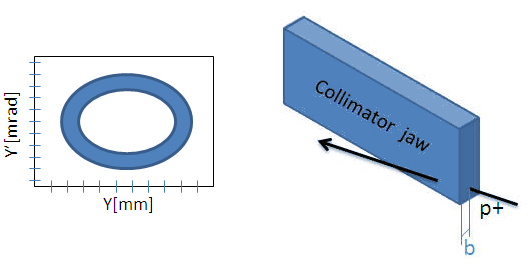
\includegraphics[width=0.5\linewidth]{figures/coll_fig1}
    \caption{\label{Coll:Fig1} \textbf{Left:} Halo particles in the phase diagram. \textbf{Right:} Impact Parameter.}
\end{center}
\end{figure}

One defines the Impact Parameter $b$ (see Figure~\ref{Coll:Fig1}) as the transverse offset between the jaw surface and the impact point.
$b$ typically equals $1\mu m$ at the first impact.

\bigskip
\noindent These changes implied to modify/add some input files:
\begin{itemize}
    \item the generic SixTrack parameter file \texttt{fort.3} now has a new block for collimation parameters,
    \item a separate collimator database file is now mandatory if collimation studies are to be done.
\end{itemize}

This database including the name, length, orientation and material of every single collimator of the ring (1 file per Collimation System Phase though).
Apart from these two, the other required SixTrack files are produced via MAD-X and its conversion module.

% ================================================================================================================================ %

\subsection{Collimation Input Block} \label{sec:coll:input}

The collimation module is controlled by the \texttt{COLL} block in \texttt{fort.3}\index{collimation}.

\bigskip
\begin{tabular}{@{}lp{0.8\linewidth}}
    \textbf{Keyword}    & \texttt{COLL}\index{COLL} \\
    \textbf{Data lines} & Either 17 lines (old format), or free (new format)\\
    \textbf{Format}     & See below.
\end{tabular}

\paragraph{Format Description:}~\\

From SixTrack version 5.2.5 and on, the main format of the \texttt(COLL) block is a set of keyword/value lines.

For backwards compatibility, the old format is still supported, and it is described in Section~\ref{sec:coll:oldfmt}.
When encountering the \texttt{COLL} block, the parser will check if the first line of the block is a single value, and if it is, it will conclude that the block is in the old format.
The old block format consists of 17 lines of varying number of values, and the full description is laid out in Table~\ref{tab:COLL_INP}.

Note that the old and new format cannot be inter-mixed.
The old format is parsed based on the line number, and must follow exactly the format described in Table~\ref{tab:COLL_INP}.

The keyword/value formated block is described below.
The keywords mostly correspond to the keywords listed in Table~\ref{tab:COLL_INP}.

\paragraph{Do Collimation (Required)} \texttt{DO\_COLL true|false}\\

The collimation module can be switched on and off in its entirety with this flag, without having to comment in and out the entire block.
When the flag is off, the collimation routines are skipped in tracking, and the additional memory needed for collimation is not allocated.
This entry is required for collimation to be enabled, but if ommitted, defaults to \texttt{false}.

\paragraph{Collimator Database (Required)} \texttt{COLLDB filename}\\

The filename of the database of collimators.
This entry is required.
The format of the database is described in Section~\ref{Sec:CollDB}.
It is also possible to load the old style database format.
If so, a converted database is written to the simulation folder with an added file extension \texttt{.new}.

\paragraph{Beam Energy (Required)} \texttt{ENERGY energy[MeV]}\\

The energy of the beam to be tracked.
This is independent of the energy specified in other blocks, and is a required value.

\paragraph{Emittance (Required)} \texttt{EMIT eX\_d eY\_d eX\_g eY\_g}\\

Specifies the normalised emittance for the distribution \texttt[eX\_d, eY\_d], and for the collimator gaps \texttt[eX\_g, eY\_g].
These are required.

\paragraph{Random Seed} \texttt{SEED seed}\\

Set the seed for the random number generator.
If set to 0 (default) a new seed will be selected for each run.

\paragraph{Distribution Generator Type} \texttt{DIST\_TYPE 0-6}\\

The type of the distribution generator to use\index{beam distribution}.
Setting this to larger than 0 will overwrite the distribution generated by the initialisation routines in SixTrack, including the distribution read from the \texttt{DIST} block (see Section~\ref{distBlock}).
This feature will be deprecated in the future, and the functionality taken over by an extended \texttt{DIST} module.
The different options are listed below.
The default value is 0.

\begin{enumerate}
    \setcounter{enumi}{-1}
    \item The internal collimation distribution generator is disabled and the general SixTrack distribution is used instead (default).
    \item Distribution in the plane for which the parameters are specified ONLY: flat distribution in the selected plane between $A_x \pm \delta A_x$ (horizontal) or $A_y \pm \delta A_y$ (vertical). The amplitude in the other plane is zero\index{beam distribution}. The parameters must be provided with the \texttt{DIST\_PARAM} keyword. Values 1 to 4 are used.
    \item Distribution in the plane for which the parameters are specified + a Gaussian distribution cut at $3\sigma$ in the other plane. The parameters must be provided with the \texttt{DIST\_PARAM} keyword. Values 1 to 4 are used.
    \item Distribution in the plane for which the parameters are specified + a Gaussian distribution cut at $3\sigma$ in the other plane. The parameters must be provided with the \texttt{DIST\_PARAM} keyword. Values 1 to 4 are used. In addition an energy spread is given as value 5, and a longitudinal component given by value 6.
    \item Reads an external file that contains the beam distribution to be tracked. The file is specified by \texttt{DIST\_FILE}.
    \item Radial transverse distribution of radius $A_r$. This corresponds to a flat distribution both in the horizontal and vertical planes between $A_x \pm \delta A_x$ and $A_y \pm \delta A_y$, with $A_x = A_y = A_r/\ddot{O}2$.
    \item Reads a normalised distribution from an external file. The file is specified by \texttt{DIST\_FILE}.
\end{enumerate}

\paragraph{Distribution Generator Parameters} \texttt{DIST\_PARAM $A_x$ $\delta A_x$ $A_y$ $\delta A_y$ [enerror bunchlen]}\\

The parameters for the distribution generator \texttt{DIST\_TYPE}.
The required values are determined by the type selected.
All values default to 0.

Recomended values are $3.06 \times 10^{-4}$ at 450 GeV and $1.129 \times 10^{-4}$ at 7 TeV for energy error (\texttt{enerror}), and 11.24 cm at 450 GeV and 7.55 cm at 7TeV for bunch length (\texttt{bunchlen}).

\paragraph{Distribution Generator Input File} \texttt{DIST\_FILE filename}\\

Name of the distribution file to be read in for distribution type 4 or 6.

\paragraph{Special Radial Distribution} \texttt{DO\_RADIAL true|false amp smear}\\

Alternative radial beam distribution where \texttt{amp} is the amplitude of the beam in numbers of radial sigmas, and \texttt{smear} is the smear of the beam in radial sigma.
Setting this to true will override \texttt{DIST\_TYPE}.

This distribution is equivalent to \texttt{DIST\_TYPE = 1} with the \texttt{DIST\_PARAM} values:
\begin{align*}
   A_x = A_y &= \mbox{\texttt{amp}}/\sqrt{2}\\
   \delta A_x = \delta A_y &= \mbox{\texttt{smear}}/\sqrt{2}
\end{align*}.

\paragraph{Special Radial Distribution} \texttt{DO\_MINGAP true|false}\\

If \texttt{true}, the particle distribution is generated at the collimator with the smallest gap (to be used with sheet/pencil beam).
Default value is \texttt{false}.

\paragraph{Do Change Collimator Gaps} \texttt{DO\_NSIG true|false}\\

If \texttt{true}, the collimator gaps specified in the imput block by keyword \texttt{NSIG\_FAM} are used instead of those in the collimator database file.
Default value is \texttt{false}.

\paragraph{Set Collimator Gaps} \texttt{NSIG\_FAM name collgap}\\

Family name and collimator gap in units of sigma for each collimator family specified below.
This is only applied to the collimators themselves if the \texttt{DO\_NSIG} is true.

The collimator family name is extracted from the collimator name in the collimator database.
The default collimator families are listed below.
A new collimation database format will be added in the near future where the families can be specified independently in the database, and not locked to the naming convention for the LHC.

The default value is the sigma gap specified in the collimator database.

\bigskip
\begin{longtabu}{@{}ll}
    \texttt{tcp3}    & The primary collimator\index{primary collimator} in IR3. \\
    \texttt{tcsg3}   & The secondary graphite collimator in IR3\index{secondary collimator}. \\
    \texttt{tcsm3}   & The secondary metallic collimator in IR3\index{secondary collimator}. \\
    \texttt{tcla3}   & The active absorbers in IR3\index{absorbers}. \\
    \texttt{tcp7}    & The primary collimators\index{primary collimator} in IR7. \\
    \texttt{tcsg7}   & The secondary graphite collimator in IR7\index{secondary collimator}. \\
    \texttt{tcsm7}   & The secondary metallic collimator in IR7\index{secondary collimator}. \\
    \texttt{tcla7}   & The active absorbers collimator\index{absorbers} in IR7. \\
    \texttt{tclp}    & The physics debris collimator. \\
    \texttt{tcli}    & The absorbers for injection protection\index{absorbers}. \\
    \texttt{tcdq}    & The beam dump protection collimator\footnote{One-sided collimators (only positive x)}. \\
    \texttt{tcstcdq} & The secondary collimator dedicated to beam dump\index{secondary collimator}. \\
    \texttt{tdi}     & The injection protection collimator. \\
    \texttt{tcth1}   & The horizontal tertiary collimator in IR1\index{tertiary collimator}. \\
    \texttt{tcth2}   & The horizontal tertiary collimator in IR2\index{tertiary collimator}. \\
    \texttt{tcth5}   & The horizontal tertiary collimator in IR5\index{tertiary collimator}. \\
    \texttt{tcth8}   & The horizontal tertiary collimator in IR8\index{tertiary collimator}. \\
    \texttt{tctv1}   & The vertical tertiary collimator in IR1\index{tertiary collimator}. \\
    \texttt{tctv2}   & The vertical tertiary collimator in IR2\index{tertiary collimator}. \\
    \texttt{tctv5}   & The vertical tertiary collimator in IR5\index{tertiary collimator}. \\
    \texttt{tctv8}   & The vertical tertiary collimator in IR8\index{tertiary collimator}. \\
    \texttt{tcxrp}   & The Roman Pots\footnote{One-sided collimators (only positive x)}. \\
    \texttt{tcryo}   & The collimators in the DS regions.
\end{longtabu}

\paragraph{Jaw Slicing}~\\

This feature has been removed from the main collimation block.
The collimators or collimator families that are to be sliced are now set in the collimator database file.
See Section~\ref{Sec:CollDB}.

\paragraph{One-Sided Collimators}~\\

This feature has been removed from the main collimation block.
The collimators or collimator families that are to be treated as one-sided are now set in the collimator database file.
See Section~\ref{Sec:CollDB}.

\paragraph{Beta-Beating} \texttt{BETA\_BEAT xbeat xbeat\_phase ybeat ybeat\_phase}\\

In case of beta-beating\index{beta-beating}:

\bigskip
\begin{tabular}{@{}llp{0.7\linewidth}}
    \texttt{xbeat}        & float & Offset in $x$ for the computation of collimator. \\
    \texttt{xbeat\_phase} & float & Phase offset in $x$ for the computation of collimator. \\
    \texttt{ybeat}        & float & Offset in $y$ for the computation of collimator. \\
    \texttt{ybeat\_phase} & float & Phase offset in $y$ for the computation of collimator.
\end{tabular}

These values default to 0.

\paragraph{Pencil Beam} \texttt{PENCIL ipencil offset rmsx rmsy distr}\\

Resets original distribution to pencil beam distribution on the collimator database ID specified by \texttt{ipencil}\index{pencil beam}.
The formats are described below.
Setting \texttt{ipencil} to 0, disables this feature.
These values default to 0.

\bigskip
\begin{tabular}{@{}l|p{0.6\linewidth}}
    \texttt{distr = 0}         & \texttt{offset = 0} \\
    Pencil Beam Distribution   & \texttt{rmsx   = 0} \\
                               & \texttt{rmsy   = 0} \\
    \hline
    \texttt{distr = 0}         & \texttt{offset = }center of rectangle \\
    Rectangular Distribution   & \texttt{rmsx   = }spread of impact parameter (uniform) \\
                               & \texttt{rmsy   = }spread parallel to jaw surface \\
    \hline
    \texttt{distr = 1}         & \texttt{offset = }mean of Gaussian distribution \\
    Gaussian Distribution      & \texttt{rmsx   = }spread of impact parameter (Gaussian) \\
                               & \texttt{rmsy   = }spread parallel to jaw surface (Gaussian) \\
    \hline
    \texttt{distr = 2}         & \texttt{offset = }mean of Gaussian distribution \\
    Half Gaussian Distribution & \texttt{rmsx   = }spread of impact parameter (uniform) \\
                               & \texttt{rmsy   = }spread parallel to jaw surface (Gaussian) \\
\end{tabular}

\bigskip
\noindent\textbf{Note:} The distribution with \texttt{distr = 2} is used when wanting to simulate the loss of a magnet.

\paragraph{Dedicated Collimator Study} \texttt{DO\_SELECT true|false name}\\

Do a dedicated study of selected collimator.
This value defaults to \texttt{false}.

\paragraph{Nominal Beta} \texttt{DO\_NOMINAL true|false}\\

Switches on or off the use of design $\beta$ values of collimators.
This value defaults to \texttt{false}.

\paragraph{Emittance Drift} \texttt{EMIT\_DRIFT driftx drifty}\\

Apply an emittance drift in the $x$ and $y$ direction, respectively.
These values default to 0.

\paragraph{Alignment Errors} \texttt{ALIGNERR\_[PRIM|SEC] rms\_tilt sys\_tilt rms\_offset sys\_offset}\\

Apply errors to primary or secondary collimator tilt and offset.
These values default to 0.

\bigskip
\begin{tabular}{@{}llp{0.7\linewidth}}
    \texttt{rms\_tilt}   & float & RMS value of tilt to apply. \\
    \texttt{sys\_tilt}   & float & Systematic value of tilt to apply. \\
    \texttt{rms\_offset} & float & RMS value of offset to apply. \\
    \texttt{sys\_offset} & float & Systematic value of offset to apply.
\end{tabular}

\paragraph{Alignment Errors to Gaps} \texttt{ALIGNERR\_GAP rmserror\_gap}\\

The RMS error of collimator gap.
These values default to 0.

\paragraph{Alignment Errors Random Seed} \texttt{ALIGNERR\_SEED seed}\\

The random number seed to use for alignemnt errors.
This value defaults to 0.

\paragraph{Systilt} \texttt{SYSTILT\_ANTI true|false}\\

Deduce \texttt{SYSTILT} to \texttt{RMSTILT} instead of adding.
This value defaults to \texttt{false}.

\paragraph{Cut Sigmas} \texttt{SIGSECUT sigma\_xy sigma\_r}\\

Sigma cuts for \texttt{tracks2.dat} controlled by the \texttt{WRITE\_TRACKS} flag.
Cut in square sigmas $x$/$y$ for saving particles (e.g. 64 for a cut at 8 $\sigma_x$/$\sigma_y$).
Cut in square sigmas radial for saving particles (e.g. 90.25 for a cut at 9.5 $\sigma_r$).
These values default to 1.

\paragraph{File Write Flags} \texttt{WRITE\_* true|false}\\

Switches on or off the writing of various output files, listed below.
All flags default to \texttt{false}.

\bigskip
\begin{tabular}{@{}llp{0.7\linewidth}}
    \texttt{WRITE\_DIST}     & Writes the beam distribution to file before and after tracking. \\
    \texttt{WRITE\_IMPACT}   & Writes the impact parameters for each collimator. \\
    \texttt{WRITE\_SECOND}   & Writes a secondary halo file based on normalised amplitude. \\
    \texttt{WRITE\_AMPL}     & Writes checking files for amplitude, closed orbit. \\
    \texttt{WRITE\_EFFIC}    & Writes the efficiency files. \\
    \texttt{WRITE\_TRACKS}   & Writes secondary/tertiary halo files. \\
    \texttt{WRITE\_CRYCOORD} & Writes crystal coordinate file(s).
\end{tabular}

% ================================================================================================================================ %

\subsection{The Collimator Database}\label{Sec:CollDB}

Collimators require specific settings, which are provided in a dedicated collimator database.
The file is specified with the \texttt{COLLDB} keyword in the \texttt{COLL} block in \texttt{fort.3}.
See Section~\ref{sec:coll:input}.

Only the new database format is described in this section, but it is possible to load a file with the old format.
The old format has been deprecated due to having a single column of parameters that are not straight-forward to read (by humans) and difficult to extend with new features.
If an old database file is specified, a converted database is written with the same file name plus an added extension \texttt{.new}.
New features added to the collimation module will not be supported by the old format.

\paragraph{Database Structure}~\\

The database is split into two sections.
The first (main) section lists all the collimators and their default parameters.
The second section, separated from the first by the keyword \texttt{SETTINGS}, contains additional settings for specific collimators or families of collimators.
The second section is parsed following similar logic to the \texttt{fort.3} input block, but has a different set of keywords.
The second section is optional.

\subsubsection{Main Database Section}

The main section of the database consists of a list of collimator family declarations, followed by a list of collimators.
The family declaration is optional, but it makes it easier to assign parameters to a group of collimators instead of specifying each one individually.
In the main section, this is used to provide the default collimator opening.

The collimator family settings are povided similarly to the \texttt{NISG\_FAM} keyword in the \texttt{COLL} block in \texttt{fort.3}.
The keyword takes a family name, a collimator opening setting, and a collimator stage as input parameters.
Note that the sigma settings in \texttt{fort.3} overrides the settings of the database.

The collimator stage is not required, and defaults to \texttt{UNKNOWN}.
Each collimator stage has a number associated with it that is an exponent of 2 (se table below).
In files like \texttt{coll\_ellipse.dat} and \texttt{tracks2.dat}, the sum of these are printed, meaning the information of what collimator stages a particle (that has not been absorbed) has hit can be extracted.
Only the first three characters of the collimator stage is required, the rest of the word is optional for clarity.

\bigskip
\begin{tabular}{@{}llp{0.7\linewidth}}
    \texttt{PRIMARY}   &  1 & Primary collimators \\
    \texttt{SECONDARY} &  2 & Secondary collimators \\
    \texttt{TERTIARY}  &  4 & Tertiary collimators \\
    \texttt{OTHER}     &  8 & Any other collimator \\
    \texttt{CRYSTAL}   & 16 & Crystal collimators \\
    \texttt{UNKNOWN}   & 32 & The collimator stage is unknown (default) \\
\end{tabular}

\bigskip
The collimator key settings are provided in a table of either 6 or 8 columns.
The latter two columns are optional.
The formats are as follows:

\bigskip
\begin{tabular}{@{}llp{0.7\linewidth}}
    \texttt{elemname} & char       & The single element name of the collimator. \\
    \texttt{opening}  & char/float & The family name as defined above, or if no family, the collimator opening in units of sigma. \\
    \texttt{material} & char(4)    & The material of the collimator. \\
    \texttt{length}   & float      & The length of the collimator in metres. \\
    \texttt{angle}    & float      & The skew angle (i.e. about the longitudinal axis) of the collimator in degrees. \\
    \texttt{offset}   & float      & The offset of the collimator on the cleaning plane in metres. \\
    \texttt{beta\_x}  & float      & The Twiss $\beta_x$ of the collimator in metres (optional). \\
    \texttt{beta\_y}  & float      & The Twiss $\beta_y$ of the collimator in metres (optional). \\
\end{tabular}

\paragraph{Example}~

\begin{cverbatim}
# Families
NSIG_FAM tcp3      12.000000 PRIMARY
NSIG_FAM tcsg3     15.600000 SECODNARY
NSIG_FAM tcsm3    999.000000 SECODNARY
NSIG_FAM tcla3     17.600000 TERTIARY
# Collimators
# name          opening mat.   length[m]  angle[deg]  offset[m]    beta_x[m]    beta_y[m]
tclx.4r1.b1        tclp Iner    1.000000    0.000000   0.000000  6812.605863  4597.092632
tcl.5r1.b1         tclp CU      1.000000    0.000000   0.000000   902.616764  1935.588447
tcl.6r1.b1         tclp Iner    1.000000    0.000000   0.000000   142.965006  1166.200842
tctph.4l2.b1      tcth2 Iner    1.000000    0.000000   0.000000    84.519178   104.259232
tctpv.4l2.b1      tctv2 Iner    1.000000   90.000000   0.000000    86.619339   103.111681
tdi.4l2.b1          tdi CU      4.000000   90.000000   0.000000   144.175250    96.678174
tclia.4r2          tcli C       1.000000   90.000000   0.000000    98.565386   160.118523
tclib.6r2.b1       tcli C       1.000000   90.000000   0.000000   149.324152    63.396485
tcp.6l3.b1         tcp3 C       0.600000    0.000000   0.000000   131.520626   144.694013
tcsg.5l3.b1       tcsg3 C       1.000000    0.000000   0.000000    54.604612   298.623904
tcsg.4r3.b1       tcsg3 C       1.000000    0.000000   0.000000    26.209714   395.196297
tcsg.a5r3.b1      tcsg3 C       1.000000  170.799865   0.000000    35.867692   344.111324
tcsg.b5r3.b1      tcsg3 C       1.000000   11.400000   0.000000    45.537821   312.677533
tcla.a5r3.b1      tcla3 Iner    1.000000   90.000000   0.000000   142.529342   176.013077
tcla.b5r3.b1      tcla3 Iner    1.000000    0.000000   0.000000   151.614782   168.687046
tcla.6r3.b1       tcla3 Iner    1.000000    0.000000   0.000000   129.435749   168.706418
tcla.7r3.b1       tcla3 Iner    1.000000    0.000000   0.000000    66.935067    92.241046
tcth.6l5.b1       tcth5 CuCD    1.000000    0.000000   0.000000  1262.953872   303.824116
tctv.6l5.b1       tctv5 CuCD    1.000000   90.000000   0.000000  1322.390819   361.810773
tctxh.4l5.b1      tcth5 CuCD    1.000000    0.000000   0.000000  4673.450003  7076.790857
\end{cverbatim}

\subsubsection{Additional Collimator Settings}

Further collimator settings can be provided at the bottom of the database file separated by the \texttt{SETTINGS} keyword.
Currently, only one-sided collimators can be specified in this section.

\paragraph{One-Sided Collimators} \texttt{ONESIDED name 1|2}\\

One-sided treatment of collimators can be achieved by setting this flag.\index{one-sided collimator}
The \texttt{name} can either be a collimator name or a family name.
The last parameter specifies either jaw 1 (i.e. at $x$>0 in the collimator reference system) or jaw 2 (i.e. at $x$<0 in the collimator reference system).
If jaw 2 is selected, the collimator is rotated by 180 degrees, as only the positive $x$ side is treated when one-sided is enabled.

\bigskip
\noindent\textit{Example}
\begin{cverbatim}
SETTINGS
ONESIDED tcdqa.a4r6.b1    1
ONESIDED tcdqa.c4r6.b1    1
ONESIDED tcdqa.b4r6.b1    1
\end{cverbatim}

\paragraph{Jaw Fit Profile} \texttt{JAW\_PROFILE name fac0 [... fac5]}\\

Adds a named fit profile with factors $s_i$ up to fifth order on the form:\index{collimator jaw fit}
\begin{equation}
    P_i = A\left[s_0 + s_1 x_i + \frac{s_2 x_i^2}{L} + s_3 x_i^3 + s_4 x_i^4 + s_5 x_i^5\right]
\end{equation}
where $P_i$ is the profile of the $i$-th slice, $A$ is a scaling factor, $L$ is the length of the collimator, and
\begin{equation}
    x_i = \frac{L(i-1)}{N}
\end{equation}
where $N$ is the number of slices.
The scaling factors default to zero, and only the $0$-th order factor is required.

\paragraph{Jaw Fit} \texttt{JAW\_FIT target nslices fit1 fit2 [scale1 scale2 [recentre1 recentre2]]}\\

Apply a fit defined with \texttt{JAW\_PROFILE} to the two jaws of a \texttt{target} collimator or family of collimators.
The number of slices is required, and so are the prfoile names \texttt{fit1} and \texttt{fit2} for collimator jaw 1 and 2, respectively.
The scaling factors \texttt{scale1} and \texttt{scale2} are optional, and default to one.
It is also possible to move the collimator such that the opening corresponds to the smallest gap after the jaw fit profile has been applied.
This can be enabled by setting the logical flags \texttt{recentre1} and \texttt{recentre2} for the two jaws.
These flags default to \texttt{off}.

\bigskip
\noindent\textit{Example}
\begin{cverbatim}
SETTINGS
JAW_PROFILE FIT_A -1.0e-5 -2.4e-3 4.3e-3 -4.1e-3 1.8e-3 3.0e-4
JAW_PROFILE FIT_B -1.0e-5 -2.4e-3 4.3e-3 -4.1e-3 1.8e-3 3.0e-4
JAW_FIT tcsg7 15 FIT_A FIT_B 1.0 1.0 on on
\end{cverbatim}

\paragraph{Crystal Collimators} \texttt{CRYSTAL name Bend XDim YDim Thick Tilt MisCut Orient}\\

This flag enables the collimator or collimator family specified in \texttt{name} to be treated as a crystal collimator.\index{crystal collimator}
Crystal collimators require an additional set of parameters described in the following:

\bigskip
\begin{tabular}{@{}llp{0.7\linewidth}}
    \texttt{Bend}   & float   & Bending radius of the crystal collimator in [m]. \\
    \texttt{XDim}   & float   & Transverse dimension along the X axis of the crystal collimator in [m]. \\
    \texttt{YDim}   & float   & Transverse dimension along the Y axis of the crystal collimator in [m]. \\
    \texttt{Thick}  & float   & Thickness of the amorphous layer of the crystal collimator in [m]. \\
    \texttt{Tilt}   & float   & Tilt of the crystal collimator in [rad] with respect to its default orientation (calculated as the divergence of the beam at that location, i.e. optimal orientation for channeling). \\
    \texttt{MisCut} & float   & Miscut angle of the crystal collimator in [rad]. \\
    \texttt{Orient} & integer & Used only for Si crystal collimators. Its value is either 1 (strip crystal, 110 planes) or 2 (quasi-mosaic crystal, 111 planes). \\
\end{tabular}

\bigskip
All the parameters default to zero.
Additional details on the physics principles of crystal collimation and benchmark against experimental data can be found in~\cite{crystal:1,crystal:2,crystal:3,crystal:4,crystal:5,crystal:6}.

The main output file is the \texttt{cry\_interaction.dat} file.\index{crystal interaction}
This file is enabled with the \texttt{WRITE\_CRYCOORD} flag in \texttt{fort.3}.
In addition, if the \texttt{DEBUG} flag is set in the \texttt{SETTINGS} block (see Section~\ref{STSett}), a \texttt{cry\_entrance.dat} and \texttt{cry\_exit.dat} file is written as well.\index{crystal dump}

\bigskip
\noindent\textit{Example}
\begin{cverbatim}
SETTINGS
CRYSTAL  cry.h.b1 61.54 2.0e-3 50.0e-3 0.0 0.0 0.0 1
\end{cverbatim}

% ================================================================================================================================ %

\subsection{Collimation with Geant4}

It is possible to use the particle-matter scattering physics of Geant4 within SixTrack.
To do this, the G4COLLIMATION flag must be added at build time, with an appropriate Geant4 library existing in your path.
Many standard collimation features are currently not implemented.
Particle longitudinal dynamics are also not currently implemented.
The \texttt{GNT4} block specified below must be used in addition to the standard collimation block in the standard \texttt{fort.3} file. \index{GNT4} \index{Geant4}

\bigskip
\begin{tabular}{@{}lp{0.8\linewidth}}
    \textbf{Keyword}    & \texttt{GNT4}\index{GNT4} \\
    \textbf{Data lines} & Variable, see below. \\
    \textbf{Format}     & This module uses a keyword, value format. See below.
\end{tabular}

\bigskip

\paragraph{Select Physics List} \texttt{PHYSICS phys}\\

The \texttt{PHYSICS} flag selects which physics list to use in Geant4.
If no flag is specified, the simulation will default to FTFP\_BERT.
Any Geant4 physics list is allowed.
Please see \url{http://geant4-userdoc.web.cern.ch/geant4-userdoc/UsersGuides/PhysicsListGuide/html/index.html} for more details.

\bigskip
\begin{tabular}{@{}llp{0.7\linewidth}}
    \texttt{phys} & char    & The name of the physics list to use.
\end{tabular}

\paragraph{Select Particles to Return to SixTrack} \texttt{RETURN type}\\

The \texttt{RETURN} flag selects which types of particles to return back to SixTrack after performing collimation.
Only charged particles are returned; neutral particles are always killed.
Possible options are \texttt{STABLE}, which will return all stable particles, \texttt{IONS}, which takes back all ions (not including protons), and to specify by individual PDG id numbers.
Both particles and anti-particles should be specified separately.
Multiple copies of the \texttt{RETURN} flag can be used to precisely select which particles are of interest.

If no flag is specified, all particles are returned, including ones that should decay.

\bigskip
\begin{tabular}{@{}llp{0.7\linewidth}}
    \texttt{type} & char/int & The particles to send back to SixTrack after tracking through Geant4.
\end{tabular}

\paragraph{Select Relative Energy Cut} \texttt{RELENERGYCUT cut}\\

The \texttt{RELENERGYCUT} flag selects an energy cut as a fraction of the energy of the reference particle.
For example, 0.5 will cut at half the energy of the reference particle.

\bigskip
\begin{tabular}{@{}llp{0.7\linewidth}}
    \texttt{cut} & float    & The cut value to use.
\end{tabular}

\paragraph{Select Absolute Energy Cut} \texttt{ABSENERGYCUT cut}\\

The \texttt{ABSENERGYCUT} flag selects an absolute energy cut, and if a particle's energy goes below this value, it will be killed.
This value is specified in GeV.

\bigskip
\begin{tabular}{@{}llp{0.7\linewidth}}
    \texttt{cut} & float    & The cut value to use in GeV.
\end{tabular}

\paragraph{Select Range Cut} \texttt{RANGECUT\_MM cut}\\

The \texttt{RANGECUT\_MM} flag selects a range cut for particle production in Geant4.
This value is specified in mm.
The unit of this cut may change in the future.

\bigskip
\begin{tabular}{@{}llp{0.7\linewidth}}
    \texttt{cut} & float    & The cut value to use in mm.
\end{tabular}

\paragraph{Enable Debugging Output} \texttt{DEBUG}\\

The \texttt{DEBUG} flag enables some additional debugging output in Geant4.
Warning: the level of output can be very verbose with a large number of particles.

% ================================================================================================================================ %

\subsection{Old Input Format}\label{sec:coll:oldfmt}

The old input block format is illustrated in the following example, and the associated variable which each value is described in Table~\ref{tab:COLL_INP}.

\bigskip
\begin{cverbatim}
COLLIMATION
   .true.
   50   7000000
   3  5  0.958  0.0015  0.0  0.0  "nothing"  1.0 129e-4  75.5
   .true.  15.0  18.0  18.0  20.0  6.0  7.0  7.0  10.0 1 0.0  999.0  8.0   7.5   999.0
   8.3  8.3  8.3  8.3  8.3  8.3  8.3  8.3  5.0 15.0
   0 19789.0  20150.0  1  1
  -1.3899e-6  -9.345e-5  5.05324e-3  -1.6595e-2  2.15955e-2  -9.96261e-3  1.0
  -1.3899e-6  -9.345e-5  5.05324e-3  -1.6595e-2  2.15955e-2  -9.96261e-3  1.0
   0.503E-09  0.503E-09
  .false. .false. 0 .true. TCP.C6L7.B1 .false. .true. .true. .true. .true.
   0.0 0.0 0.0 0.0
   0   0   0   0   0   0   0   0   0   0   .false.
  .false.  6.003  0.0015
   0.0 0.0 .false. .false.
   0   0.0025  0.0   0.0   0
   "CollDB_V6.500_lowb_st.b1.data"  1
   .true. .false. WAbsVertLowbcoll  101  1  1.
NEXT
\end{cverbatim}

\paragraph{Old Collimator Database Format}~\\

The collimator database is stored in files named \texttt{CollDB\_V6.500\_[type]\_st.[beam].data}, with \texttt{[type]} being either inj for injection case or low $b$ for collision case, and \texttt{[beam]} being $b1$ or $b2$.
These files contain mechanical and optical data related to the collimators planned for LHC. (Note that at present only Phase I collimators have a length different from zero)

A sample block of either one of these input files follows:

\begin{cverbatim}
TCP.D6L7.B1             <-- collimator name in capital letters
tcp.d6l7.b1             <-- collimator name in minimal letters
5.7                     <-- collimator nominal opening (in sigma units)
C                       <-- collimator material (C = graphite, CU = copper, W=tungsten)
  0.2000000000000000    <-- collimator length [m]
  1.5710000000000000    <-- collimator angle [rad]
  0.0000000000000000    <-- collimator offset [m]
 90.4467000000000070    <-- design Beta x [m]
156.4360000000000070    <-- design Beta y [m]
#                       <-- line jump to next block
\end{cverbatim}

The introduction of the optic parameter $\beta$ allows studies of error scenarios (orbit distortion, beta-beating\index{beta-beating}) and/or to see the effect of misaligned collimators.
This structure is then repeated within the file for each of the collimators to be included in the study.

\bigskip
\begin{center}
\begin{longtable}{| p{0.5cm} | p{2.4cm} | p{1.2cm} | >{\raggedright\arraybackslash}p{11.4cm}|}
    \caption{Old Collimation Input Format}
    \label{tab:COLL_INP} \\*
    \hline
    \rowcolor{blue!30}
    Ln & Keyword & Type & Description \\*
    \hline
    \endfirsthead

    \hline
    \rowcolor{blue!30}
    Ln & Keyword & Type & Description \\*
    \hline
    \endhead

    \rowcolor{gray!15}
    \multicolumn{4}{|c|}{(The table continues on the next page)}\\*
    \hline
    \endfoot

    \hline
    \endlastfoot

    1   & \texttt{DO\_COLL}      & logical & Switches on/off the collimation studies. \\
    \hline

    2   & \texttt{NLOOP}         & integer & Number of samples. No longer in use. Fixed to 1. \\
        \cline{2-4}
        & \texttt{MYENOM}        & float   & Energy of the beam to be tracked. \\
    \hline

    3   & \texttt{DO\_THISDIS}   & integer & Selects the type of distribution of the particles to be tracked (see below). \\
        \cline{2-4}
        & \texttt{MYNEX}         & float   & $A_x$ normalized amplitude of particles (in sigma units) in the $x$ direction. \\
        \cline{2-4}
        & \texttt{MDEX}          & float   & $\mbox{d}A_x$ smear (in sigma units) of the beam halo around $A_x$ (in $x$ direction). \\
        \cline{2-4}
        & \texttt{MYNEY}         & float   & $A_y$ normalized amplitude of particles (in sigma units) in the $y$ direction. \\
        \cline{2-4}
        & \texttt{MDEY}          & float   & $\mbox{d}A_y$ smear (in sigma units) of the beam halo around $A_y$ (in $y$ direction). \\
        \cline{2-4}
        & \texttt{FILENAME\_DIS} & char    & Name of the distribution file to be read if \texttt{DO\_THISDIS = 4/6}. \\
        \cline{2-4}
        & \texttt{ENERROR}       & float   & Energy spread of the tracked beam. Read only if \texttt{DO\_THISDIS = 3}. \\
        \cline{2-4}
        & \texttt{BUNCHLENGTH}   & float   & Bunch length of the tracked beam in millimeters. Read only if \texttt{DO\_THISDIS = 3}. \\
    \hline

    4   & \texttt{DO\_NSIG}      & logical & If TRUE use collimators settings from \texttt{fort.3}. If FALSE from \texttt{CollDB\_V6.500\_[type]\_st.[beam].data}. \\
        \cline{2-4}
        & \texttt{NSIG\_TCP3}    & float   & Opening of the primary collimator\index{primary collimator} in IR3 in sigma units. \\
        \cline{2-4}
        & \texttt{NSIG\_TCSG3}   & float   & Opening of the secondary graphite collimator in IR3 in sigma units\index{secondary collimator}. \\
        \cline{2-4}
        & \texttt{NSIG\_TCSM3}   & float   & Opening of the secondary metallic collimator in IR3 in sigma units\index{secondary collimator}. \\
        \cline{2-4}
        & \texttt{NSIG\_TCLA3}   & float   & Opening of the active absorbers in IR3 in sigma units\index{absorbers}. \\
        \cline{2-4}
        & \texttt{NSIG\_TCP7}    & float   & Opening of the primary collimators\index{primary collimator} in IR7 in sigma units. \\
        \cline{2-4}
        & \texttt{NSIG\_TCSG7}   & float   & Opening of the secondary graphite collimator in IR7 in sigma units\index{secondary collimator}. \\
        \cline{2-4}
        & \texttt{NSIG\_TCSM7}   & float   & Opening of the secondary metallic collimator in IR7 in sigma units\index{secondary collimator}. \\
        \cline{2-4}
        & \texttt{NSIG\_TCLA7}   & float   & Opening of the active absorbers collimator\index{absorbers} in IR7 in sigma units. \\
        \cline{2-4}
        & \texttt{NSIG\_TCLP}    & float   & Opening of the physics debris collimator in sigma units. \\
        \cline{2-4}
        & \texttt{NSIG\_TCLI}    & float   & Opening of the absorbers for injection protection in sigma units\index{absorbers}. \\
        \cline{2-4}
        & \texttt{NSIG\_TCDQ}    & float   & Opening of the beam dump protection collimator in sigma units\footnote{One-sided collimators (only positive x)}. \\
        \cline{2-4}
        & \texttt{NSIG\_TCSTCDQ} & float   & Opening of secondary collimator dedicated to beam dump in sigma units\index{secondary collimator}. \\
        \cline{2-4}
        & \texttt{NSIG\_TDI}     & float   & Opening of the injection protection collimator in sigma units. \\
    \hline

    5   & \texttt{NSIG\_TCTH1}   & float   & Opening of the horizontal tertiary collimator in IR1 in sigma units\index{tertiary collimator}. \\
        \cline{2-4}
        & \texttt{NSIG\_TCTH2}   & float   & Opening of the horizontal tertiary collimator in IR2 in sigma units\index{tertiary collimator}. \\
        \cline{2-4}
        & \texttt{NSIG\_TCTH5}   & float   & Opening of the horizontal tertiary collimator in IR5 in sigma units\index{tertiary collimator}. \\
        \cline{2-4}
        & \texttt{NSIG\_TCTH8}   & float   & Opening of the horizontal tertiary collimator in IR8 in sigma units\index{tertiary collimator}. \\
        \cline{2-4}
        & \texttt{NSIG\_TCTV1}   & float   & Opening of the vertical tertiary collimator in IR1 in sigma units\index{tertiary collimator}. \\
        \cline{2-4}
        & \texttt{NSIG\_TCTV2}   & float   & Opening of the vertical tertiary collimator in IR2 in sigma units\index{tertiary collimator}. \\
        \cline{2-4}
        & \texttt{NSIG\_TCTV5}   & float   & Opening of the vertical tertiary collimator in IR5 in sigma units\index{tertiary collimator}. \\
        \cline{2-4}
        & \texttt{NSIG\_TCTV8}   & float   & Opening of the vertical tertiary collimator in IR8 in sigma units\index{tertiary collimator}. \\
        \cline{2-4}
        & \texttt{NSIG\_TCXRP}   & float   & Opening of the Roman Pots in sigma units\footnote{One-sided collimators (only positive x)}. \\
        \cline{2-4}
        & \texttt{NSIG\_TCRYO}   & float   & Opening of the collimators in the DS regions in sigma units. \\
    \hline

    6   & \texttt{N\_SLICES}     & float   & Surface model of the jaw: number of slices in which each jaw should be cut. \\
        \cline{2-4}
        & \texttt{SMIN\_SLICES}  & float   & Surface model of the jaw: s position for the start of the slicing. \\
        \cline{2-4}
        & \texttt{SMAX\_SLICES}  & float   & Surface model of the jaw: s position for the end of the slicing. \\
        \cline{2-4}
        & \texttt{RECENTER1}     & float   & Surface model of the jaw: moving the 1st jaw to the new smallest opening. \\
        \cline{2-4}
        & \texttt{RECENTER2}     & float   & Surface model of the jaw: moving the 2nd jaw to the new smallest opening. \\
    \hline

    7   & \texttt{FIT1\_1}       & float   & Surface model of the jaw: Polynomial fit 0th order for the 1st jaw. \\
        \cline{2-4}
        & \texttt{FIT1\_2}       & float   & Surface model of the jaw: Polynomial fit 1st order for the 1st jaw. \\
        \cline{2-4}
        & \texttt{FIT1\_3}       & float   & Surface model of the jaw: Polynomial fit 2nd order for the 1st jaw. \\
        \cline{2-4}
        & \texttt{FIT1\_4}       & float   & Surface model of the jaw: Polynomial fit 3rd order for the 1st jaw. \\
        \cline{2-4}
        & \texttt{FIT1\_5}       & float   & Surface model of the jaw: Polynomial fit 4th order for the 1st jaw. \\
        \cline{2-4}
        & \texttt{FIT1\_6}       & float   & Surface model of the jaw: Polynomial fit 5th order for the 1st jaw. \\
        \cline{2-4}
        & \texttt{SSF1}          & float   & Surface model of the jaw: Polynomial fit scaling for the 1st jaw. \\
    \hline

    8   & \texttt{FIT2\_1}       & float   & Surface model of the jaw: Polynomial fit 0th order for the 2nd jaw. \\
        \cline{2-4}
        & \texttt{FIT2\_2}       & float   & Surface model of the jaw: Polynomial fit 1st order for the 2nd jaw. \\
        \cline{2-4}
        & \texttt{FIT2\_3}       & float   & Surface model of the jaw: Polynomial fit 2nd order for the 2nd jaw. \\
        \cline{2-4}
        & \texttt{FIT2\_4}       & float   & Surface model of the jaw: Polynomial fit 3rd order for the 2nd jaw. \\
        \cline{2-4}
        & \texttt{FIT2\_5}       & float   & Surface model of the jaw: Polynomial fit 4th order for the 2nd jaw. \\
        \cline{2-4}
        & \texttt{FIT2\_6}       & float   & Surface model of the jaw: Polynomial fit 5th order for the 2nd jaw. \\
        \cline{2-4}
        & \texttt{SSF2}          & float   & Surface model of the jaw: Polynomial fit scaling for the 2nd jaw. \\
    \hline

    9   & \texttt{DISTEMITX0}    & float   & Normalised emittance in the horizontal plane for distribution. \\
        \cline{2-4}
        & \texttt{DISTEMITY0}    & float   & Normalised emittance in the vertical plane for distribution. \\
        \cline{2-4}
        & \texttt{COLGAPEMITX0}  & float   & Normalised emittance in the horizontal plane for collimator gaps. \\
        \cline{2-4}
        & \texttt{COLGAPEMITY0}  & float   & Normalised emittance in the vertical plane for collimator gaps. \\
    \hline

    10  & \texttt{DO\_SELECT}    & logical & Does dedicated study of selected collimator, see \texttt{NAME\_SEL}. \\
        \cline{2-4}
        & \texttt{DO\_NOMINAL}   & logical & Switches on/off the use of design $\beta$ values of collimators. \\
        \cline{2-4}
        & \texttt{RND\_SEED}     & integer & Seed studied. If set to 0, seed will be selected from system clock for every run. \\
        \cline{2-4}
        & \texttt{DOWRITE\_DIST} & logical & Saves the initial distribution to be tracked. \\
        \cline{2-4}
        & \texttt{NAME\_SEL}     & char    & Name as in the \texttt{fort.2} file of the collimator one wants a dedicated study. \\
        \cline{2-4}
        & \texttt{DO\_ONESIDE}   & logical & Switches on/off all TCPs being one-sided. Only positive jaw. If the negative jaw is to be used, it is necessary to turn collimator by 180 degrees in the collimator database file \texttt{CollDB\_V6.500\_[type]\_st.[beam].data}. \\
        \cline{2-4}
        & \texttt{DOWRT\_IMPACT} & logical & Saves the impact parameters for each collimator. \\
        \cline{2-4}
        & \texttt{DOWRT\_SECOND} & logical & Writes a secondary halo file based on normalised amplitude. \\
        \cline{2-4}
        & \texttt{DOWRT\_AMPL}   & logical & Writes checking files for amplitude, closed orbit. \\
        \cline{2-4}
        & \texttt{DOWRT\_EFFIC}  & logical & Writes the efficiency files. \\
    \hline

    11  & \texttt{XBEAT}         & float   & Offset in $x$ for the computation of collimator in case of beta-beating\index{beta-beating}. \\
        \cline{2-4}
        & \texttt{XBEATPHASE}    & float   & Phase offset in $x$ for the computation of collimator in case of beta-beating\index{beta-beating}. \\
        \cline{2-4}
        & \texttt{YBEAT}         & float   & Offset in $y$ for the computation of collimator in case of beta-beating\index{beta-beating}. \\
        \cline{2-4}
        & \texttt{YBEATPHASE}    & float   & Phase offset in $y$ for the computation of collimator in case of beta-beating\index{beta-beating}. \\
    \hline

    12  & \texttt{RMSTILT\_PRIM} & float   & RMS value of tilt to apply to primary collimators\index{primary collimator}. \\
        \cline{2-4}
        & \texttt{RMSTILT\_SEC}  & float   & RMS value of tilt to apply to secondary collimators\index{secondary collimator}. \\
        \cline{2-4}
        & \texttt{SYSTILT\_PRIM} & float   & Systematic value of tilt to apply to primary collimators.\index{primary collimator} \\
        \cline{2-4}
        & \texttt{SYSTILT\_SEC}  & float   & Systematic value of tilt to apply to secondary collimators\index{secondary collimator}. \\
        \cline{2-4}
        & \texttt{RMSOFFS\_PRIM} & float   & RMS value of offset to apply to primary collimators\index{primary collimator}. \\
        \cline{2-4}
        & \texttt{RMSOFFS\_SEC}  & float   & RMS value of offset to apply to secondary collimators\index{secondary collimator}. \\
        \cline{2-4}
        & \texttt{SYSOFFS\_PRIM} & float   & Systematic value of offset to apply to primary collimators\index{primary collimator}. \\
        \cline{2-4}
        & \texttt{SYSOFFS\_SEC}  & float   & Systematic value of offset to apply to secondary collimators\index{secondary collimator}. \\
        \cline{2-4}
        & \texttt{OFFTILT\_SEED} & float   & Random number seed to be used for the simulation. \\
        \cline{2-4}
        & \texttt{RMSERROR\_GAP} & float   & RMS error of collimator gap. \\
        \cline{2-4}
        & \texttt{DO\_MINGAP}    & logical & If TRUE the particle distribution is generated at the collimator with the smallest gap (to be used with sheet/pencil beam). \\
    \hline

    13  & \texttt{RADIAL}        & logical & Switches on/off the radial distribution. \\
        \cline{2-4}
        & \texttt{NR}            & float   & Size of the beam to be tracked in number of radial sigmas. \\
        \cline{2-4}
        & \texttt{NDR}           & float   & Smear of the beam to be tracked in number of radial sigmas. \\
    \hline

    14  & \texttt{DRIFTSX}       & float   & Apply an emittance drift\index{emittance drift} in the $x$ direction. \\
        \cline{2-4}
        & \texttt{DRIFTSY}       & float   & Apply an emittance drift\index{emittance drift} in the $y$ direction. \\
        \cline{2-4}
        & \texttt{CUT\_INPUT}    & logical & This value is no longer used, and is ignored. \\
        \cline{2-4}
        & \texttt{SYSTILT\_ANTI} & logical & Deduce \texttt{SYSTILT} to \texttt{RMSTILT} instead of adding. \\
    \hline

    15  & \texttt{IPENCIL}       & integer & Resets original distribution to pencil beam\index{pencil beam} distribution on selected collimator. \\
        \cline{2-4}
        & \texttt{PENC\_OFFSET}  & float   & Size in sigma units of the desired impact parameter. \\
        \cline{2-4}
        & \texttt{PENC\_RMSX}    & float   & See table below. \\
        \cline{2-4}
        & \texttt{PENC\_RMSY}    & float   & See table below. \\
        \cline{2-4}
        & \texttt{PENC\_DISTR}   & integer & See table below. \\
    \hline

    16  & \texttt{COLL\_DB}      & char    & Name of the collimator database. \\
        \cline{2-4}
        & \texttt{IBEAM}         & integer & This value is no longer used, and is ignored. \\
    \hline

    17  & \texttt{DOWRITETRACKS} & logical & Writes secondary/tertiary halo files. \\
        \cline{2-4}
        & \texttt{CERN}          & logical & This value is no longer used, and is ignored. \\
        \cline{2-4}
        & \texttt{CASTORDIR}     & char    & This value is no longer used, and is ignored. \\
        \cline{2-4}
        & \texttt{JOBNUMBER}     & integer & This value is no longer used, and is ignored. \\
        \cline{2-4}
        & \texttt{SIGSECUT2}     & float   & Cut in square sigmas $x$/$y$ for saving particles (e.g. 64 for a cut at 8 $\sigma_x$/$\sigma_y$). \\
        \cline{2-4}
        & \texttt{SIGSECUT3}     & float   & Cut in square sigmas radial for saving particles (e.g. 90.25 for a cut at 9.5 $\sigma_r$). \\
    \hline
\end{longtable}
\end{center}
% ================================================================================================================================ %

\section{Fringe Fields} \label{sec:ffield}

\textcolor{notered}{\textbf{Note:} This module is experimental, and not yet ready for production.}

This method allows for the usage of a longitudinal description of the quadrupole magnetic field, adapted for each magnet specifically selected for the study, without changing the reference optics of SixTrack~\cite{ffield:1,ffield:2,ffield:3}.
This Fringe Field\index{Fringe Field} module is controlled by the \texttt{FFIE} block.

\bigskip
\begin{tabular}{@{}lp{0.8\linewidth}}
    \textbf{Keyword}    & \texttt{FFIE}\index{FFIE} \\
    \textbf{Data lines} & Variable, see below. \\
    \textbf{Format}     & This module uses a keyword, value format. See below.
\end{tabular}

\bigskip

\paragraph{Select Quadrupole} \texttt{FFQN quadname in ex}\\

The \texttt{FFQN} flag selects which quadrupole (name) has a longitudinal description in additional files that will be loaded in the study and link it to the type of Fringe Field that will be used (additional file).

\bigskip
\begin{tabular}{@{}llp{0.7\linewidth}}
    \texttt{quadname} & char    & Name of quadrupole. Must be the same as in the list of single elements. \\
    \texttt{in}       & integer & Index of the fringe field to use at the beginning of the quadrupole. \\
    \texttt{ex}       & integer & Index of the fringe field to use at the end of the quadrupole.
\end{tabular}

\paragraph{Select Skipped Multipole} \texttt{FFMS multname}\\

The \texttt{FFMS} flag specify the name of the multipole to skip in the tracking, in order to not increase the integrated non-linearities if multipole kicks are already added for the quadrupole in the lattice.

\bigskip
\begin{tabular}{@{}llp{0.7\linewidth}}
    \texttt{multname} & char & Name of multipole that will be skipped in the main lattice. Must be the same as in the list of single elements.
\end{tabular}

\paragraph{Profile Files} \texttt{FFFI file length\_quad length\_tot [aperture]}\\

The \texttt{FFFI} flag is followed by the files where the different Fringe Field vector potential values are saved.
The fringe field vector potential profile is saved using the format shown in Table~\ref{tab:ffield_file}.

\bigskip
\begin{tabular}{@{}llp{0.7\linewidth}}
    \texttt{file}         & char  & Name of the fringe field profile file. See next table for proper formatting. \\
    \texttt{length\_quad} & float & Length inside the quadrupole, i.e. integrated length of the equivalent quadrupole for this file. \\
    \texttt{length\_tot}  & float & Total length of integration inside the file. \\
    \texttt{aperture}     & float & The physical aperture of the quadrupole, or the maximum apeture at which you trust the representation of the Vector Potential. This parameter is optional. By defualt it is fixed as 0.080m.
\end{tabular}

\begin{center}
\begin{longtable}{|c|c|p{11cm}|}
    \caption{Input parameter in the Fringe Field profile files.}
    \label{tab:ffield_file} \\*
    \hline
    \rowcolor{blue!30}
    Arg. & Unit & Description \\*
    \hline
    \endfirsthead

    \texttt{z} & $m$ & Longitudinal position of the kick. \\*
    \hline

    \texttt{i} & -- & Exponent of x in the Horner polynomial representation of the vector potential.  \\*
    \hline

    \texttt{j} & -- & Exponent of y in the Horner polynomial representation of the vector potential. \\*
    \hline

    \texttt{k} & -- & Exponent of z in the Horner polynomial representation of the vector potential. Always 0 in case of magnetic quadrupole. \\*
    \hline

    \texttt{Ax} & $m^{-(1+i+j)}$ & Coefficient of the Horner polynomial of the vector potential for the axis x. \\*
    \hline

    \texttt{Ay} & $m^{-(1+i+j)}$ & Coefficient of the Horner polynomial of the vector potential for the axis y. \\*
    \hline

    \texttt{Az} & $m^{-(1+i+j)}$ & Coefficient of the Horner polynomial of the vector potential for the axis z. \\*
    \hline

\end{longtable}
\end{center}
